
\section{Electronica}
	\subsection{Material necesario}
		\begin{itemize}
			\item Placa Sanguinolu.
			\item Drivers de potencia stepstick.
			\item Pines de conexion macho.
			\item Motores nema 17.
			\item Fuente de alimentación.
			\item Endstop.
			\item Cable de 5 pines.
			\item Cable de 3 pines.
			\item Cable de 2 pines.
		\end{itemize}
		\begin{figure}[!htp]
			\centering
			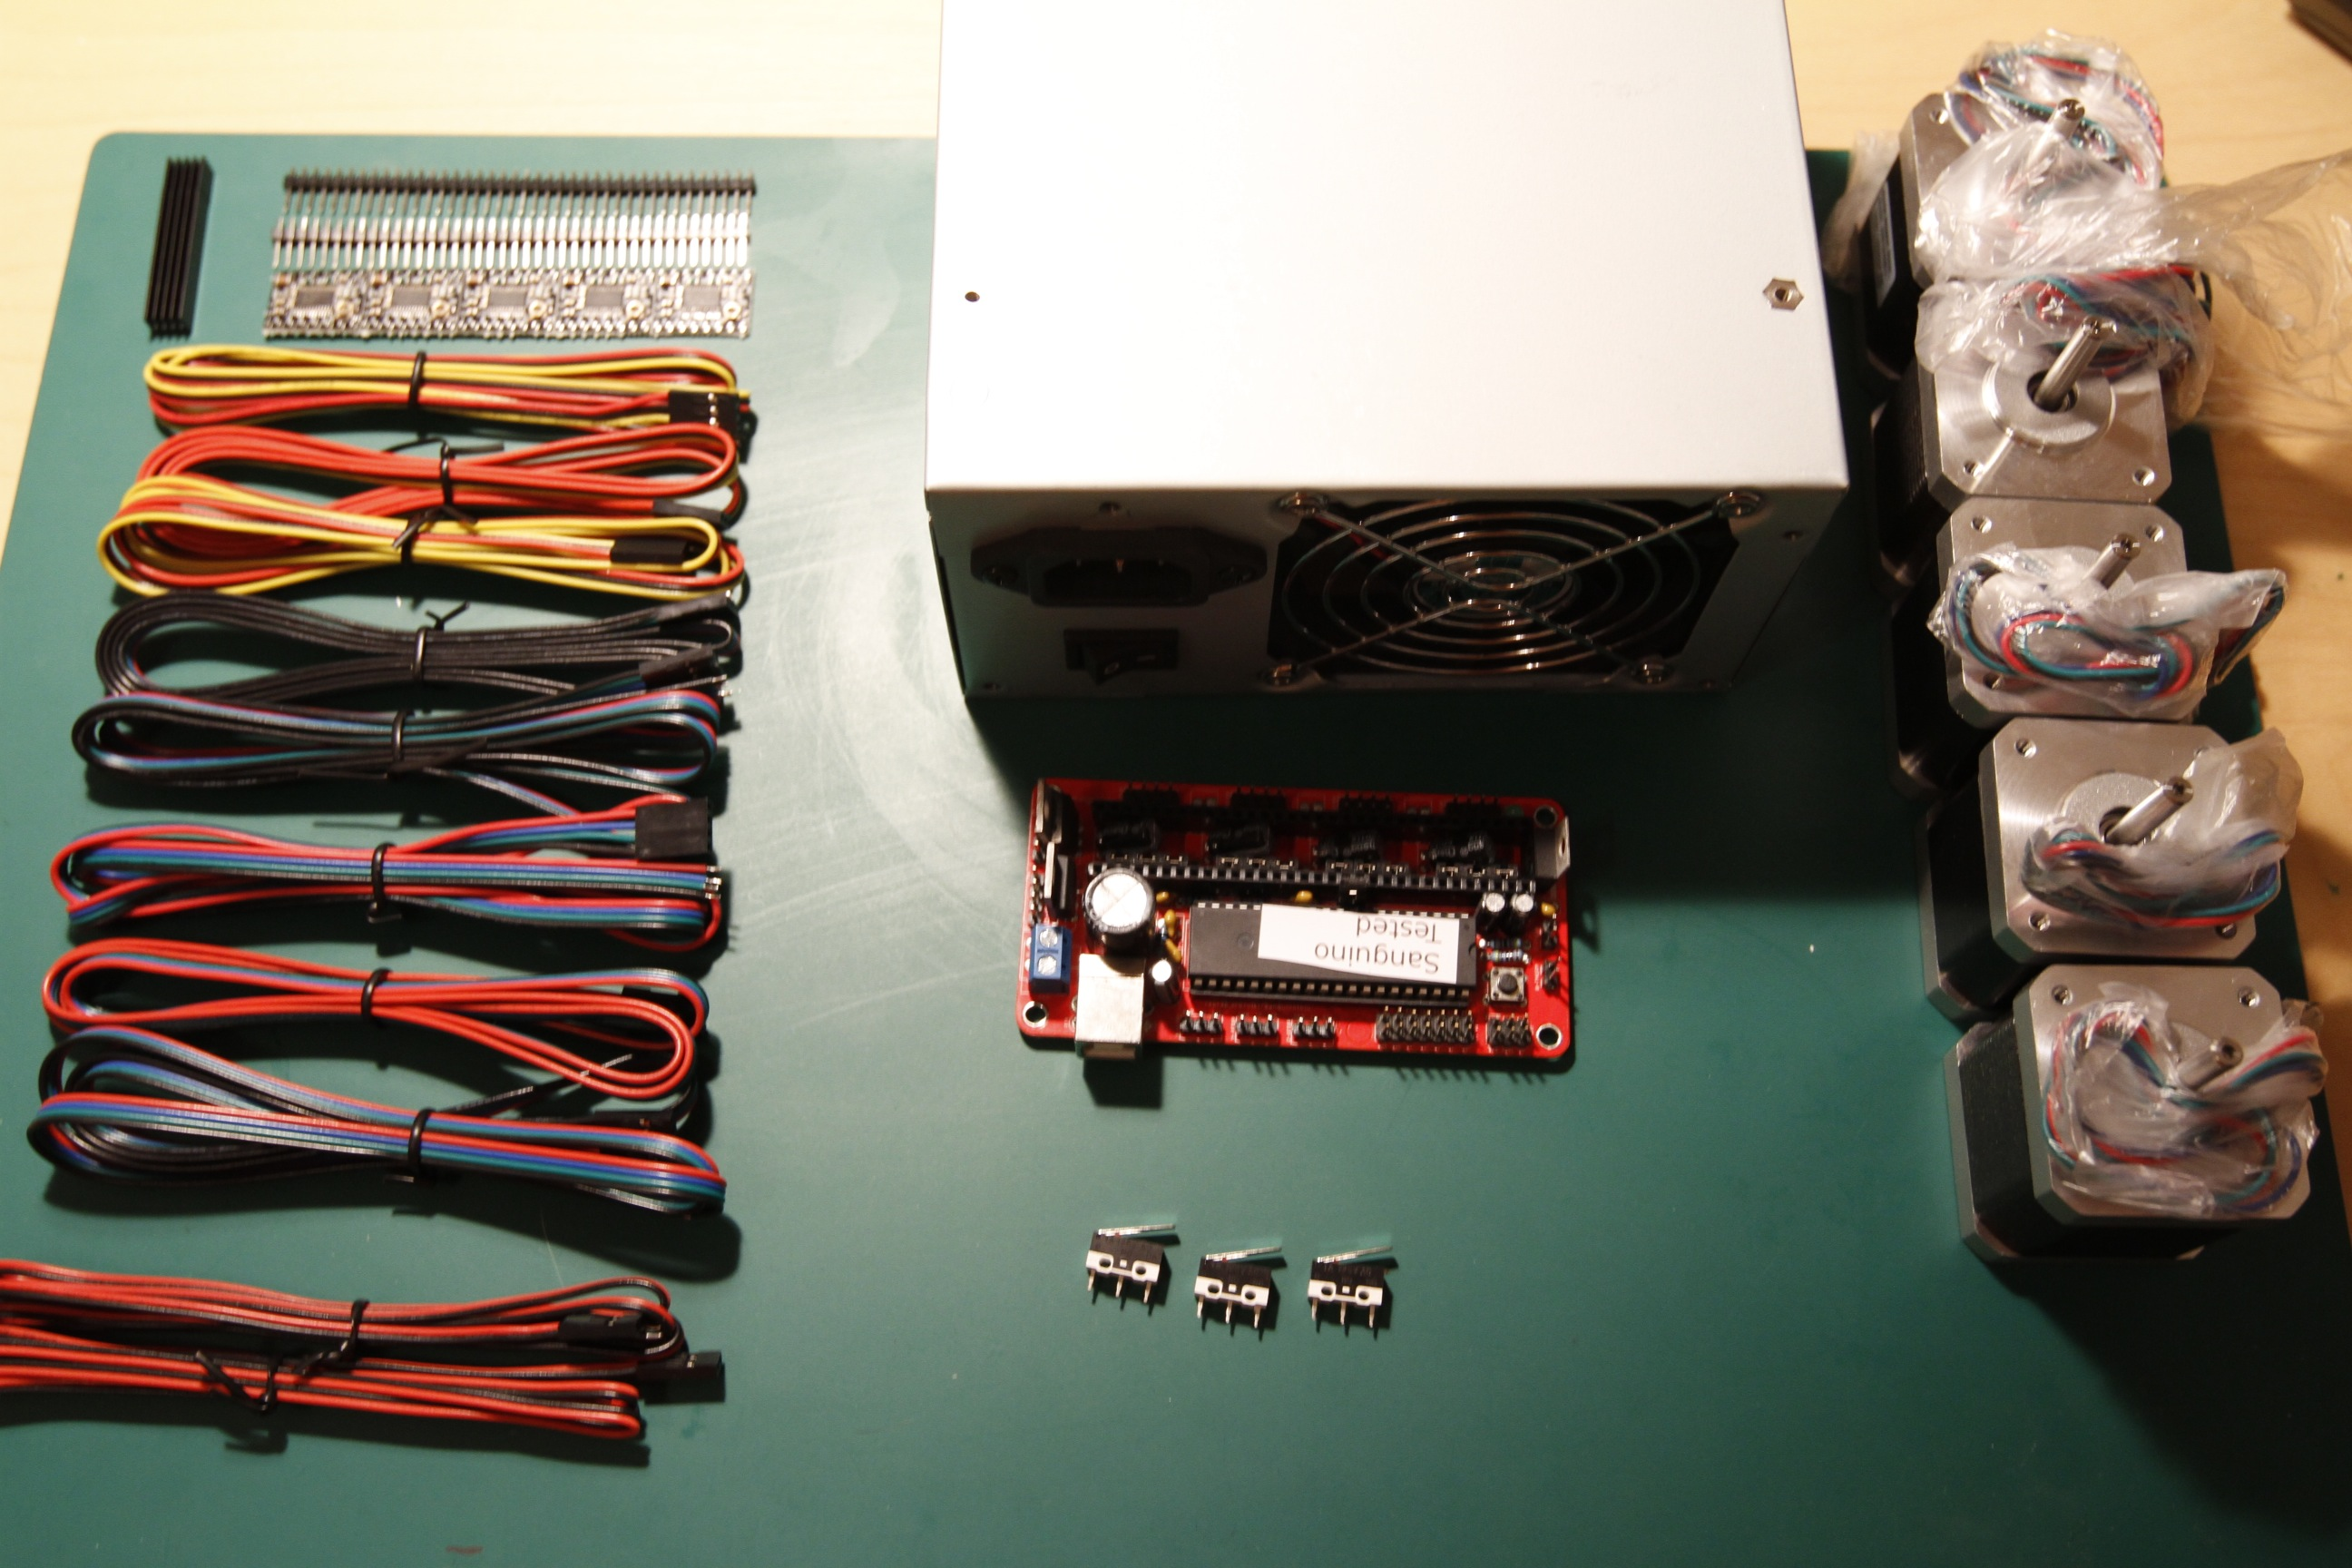
\includegraphics[width=0.7\textwidth]{../../Fotos/2.jpg}
			\caption{Material necesario}
		\end{figure}
		\newpage{}
	\subsection{Herramienta necesaria}
		\begin{itemize}
			\item Alicates de corte.
			\item Alicates de punta fina.
			\item Tijeras.
			\item Soldador.
			\item Estaño.
			\item Destornillador.
			\item Protoboard.
			\item Pinzas.	
			\item Lima fina.
		\end{itemize}
		\begin{figure}[!htp]
			\centering
			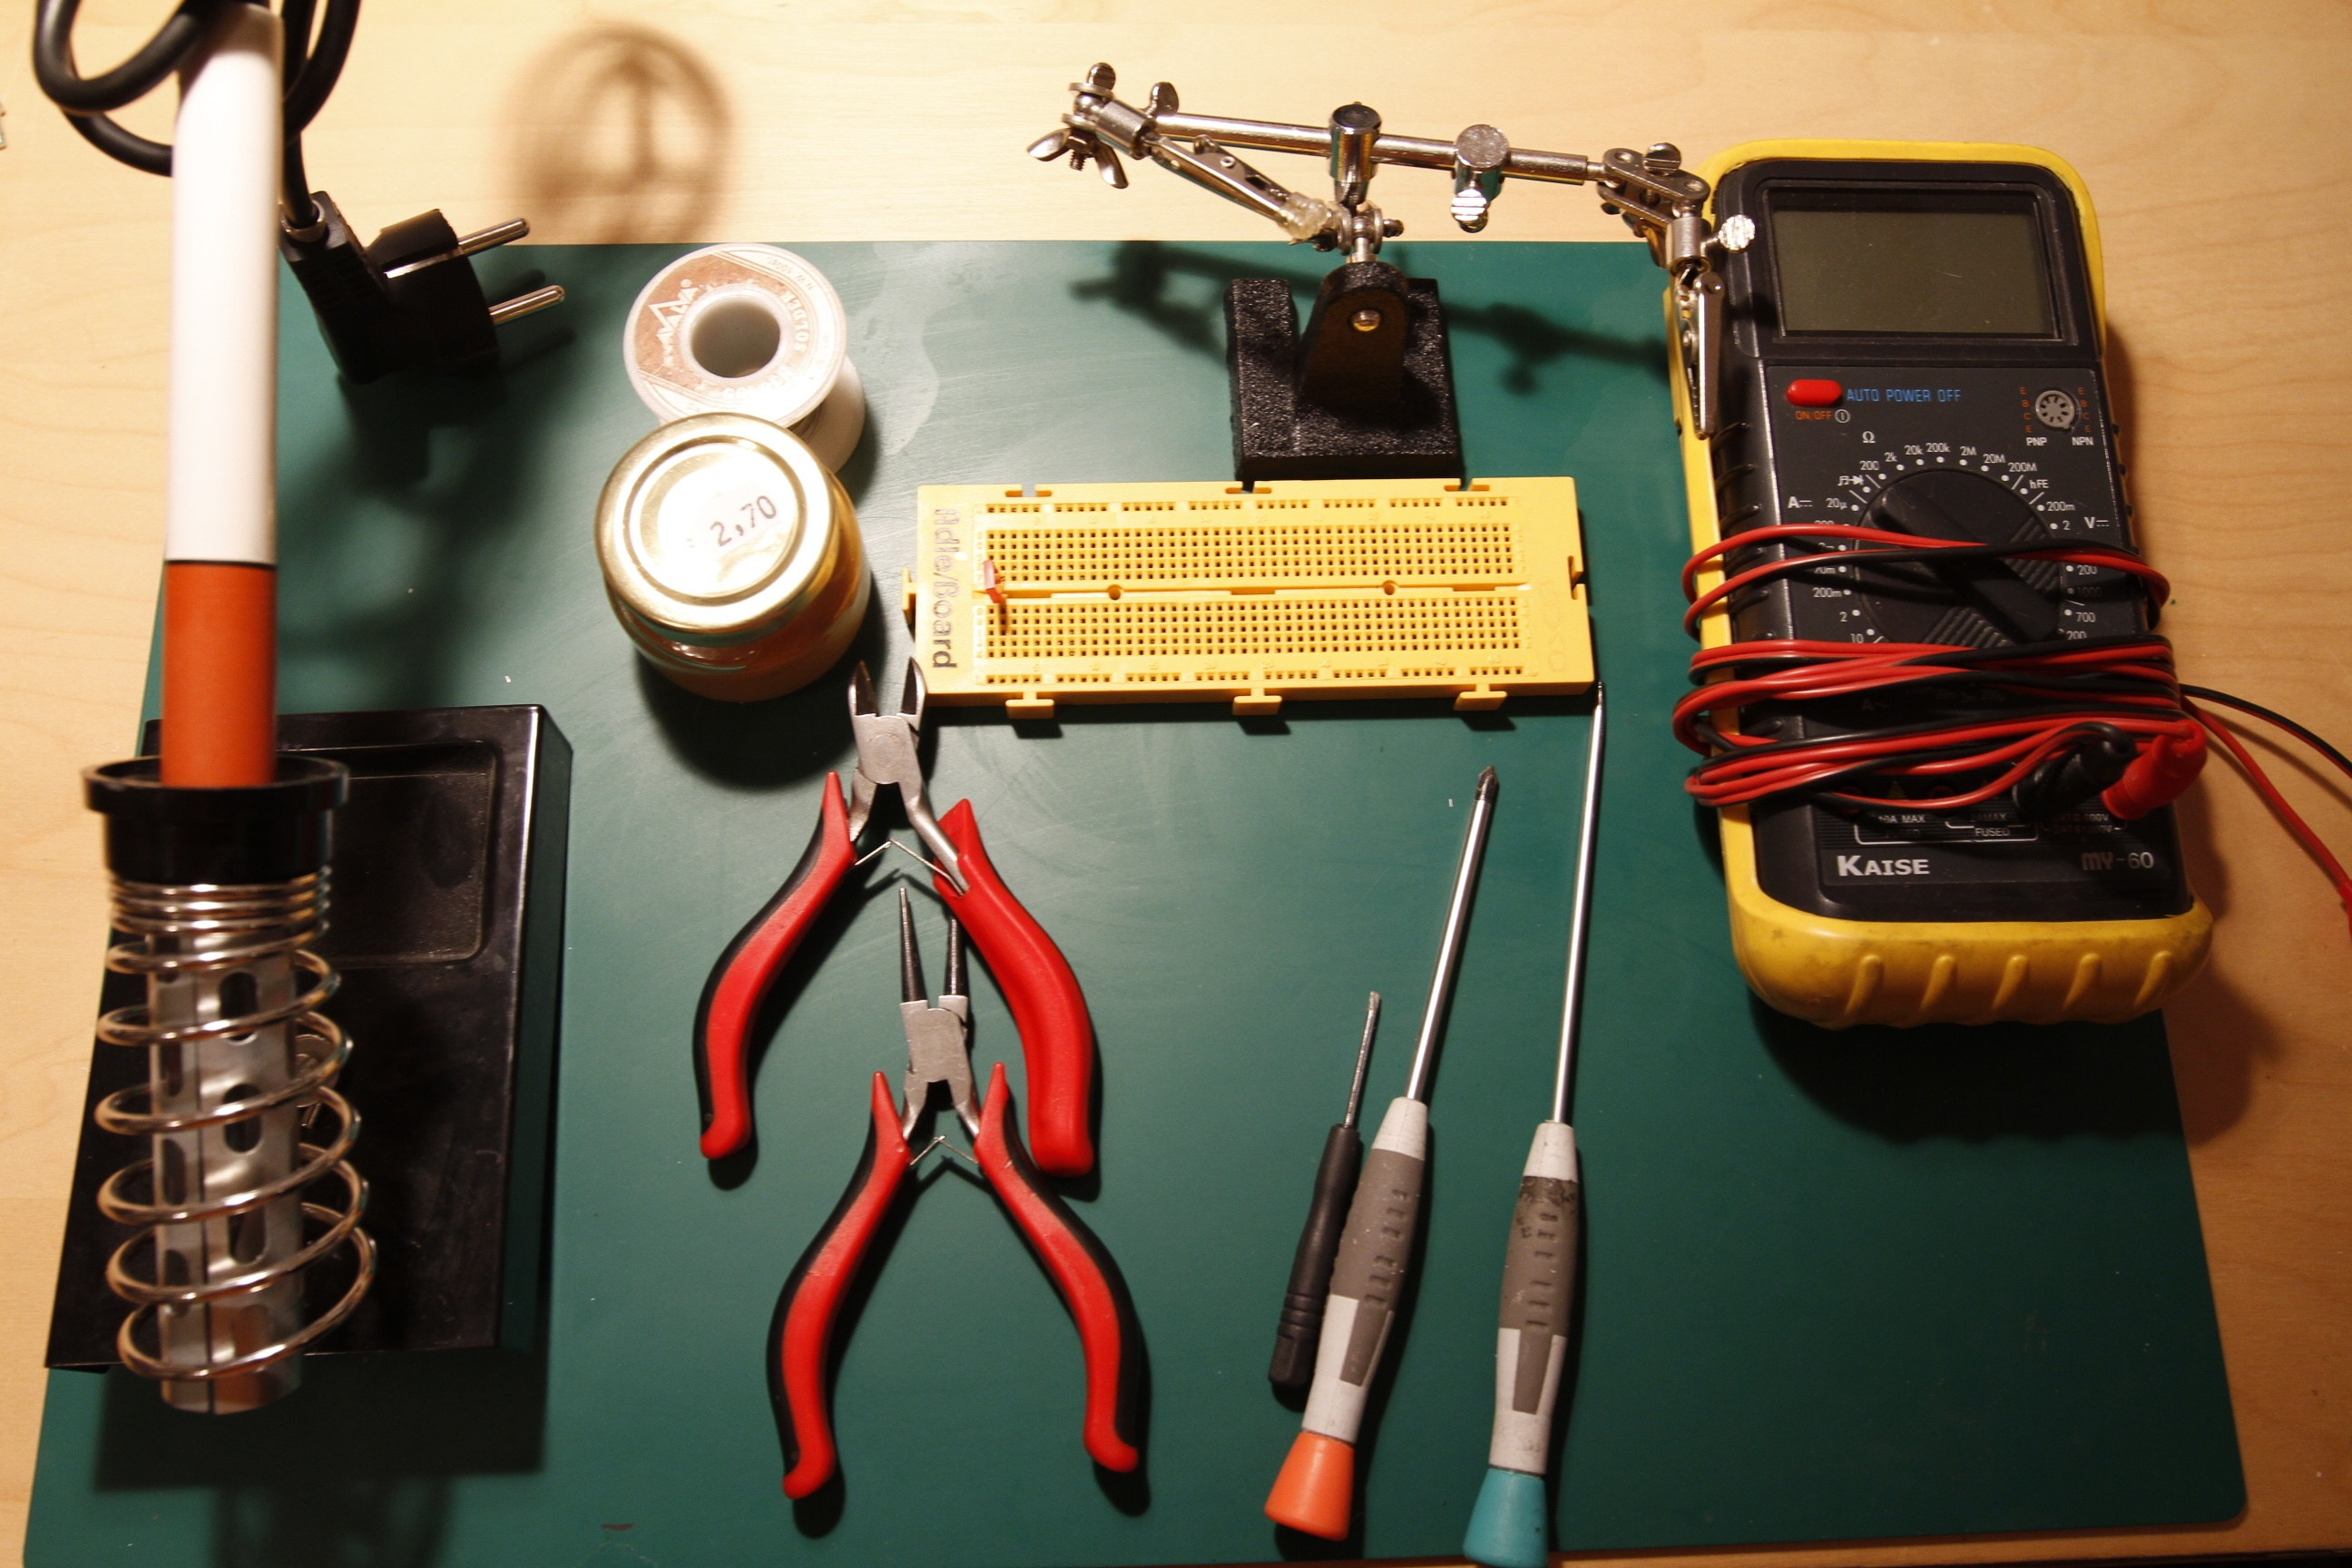
\includegraphics[width=0.7\textwidth]{../../Fotos/8.jpg}
			\caption{Herramienta necesaria}
		\end{figure}
		\newpage{}
	\subsection{Operativa}
		\subsubsection{Preprando stepsticks}
		El primer paso de todo será el soldar los pines de conexión macho a los drivers de potencia(stepsticks). Para ello deberemos separar los stepsticks como se indica en la figura ~\ref{fig:cortar.stepstick} y cortar 8 pines macho seguidos (Ver figura ~\ref{fig:cortar.pines})\\
				\begin{figure}[H]
				\centering
				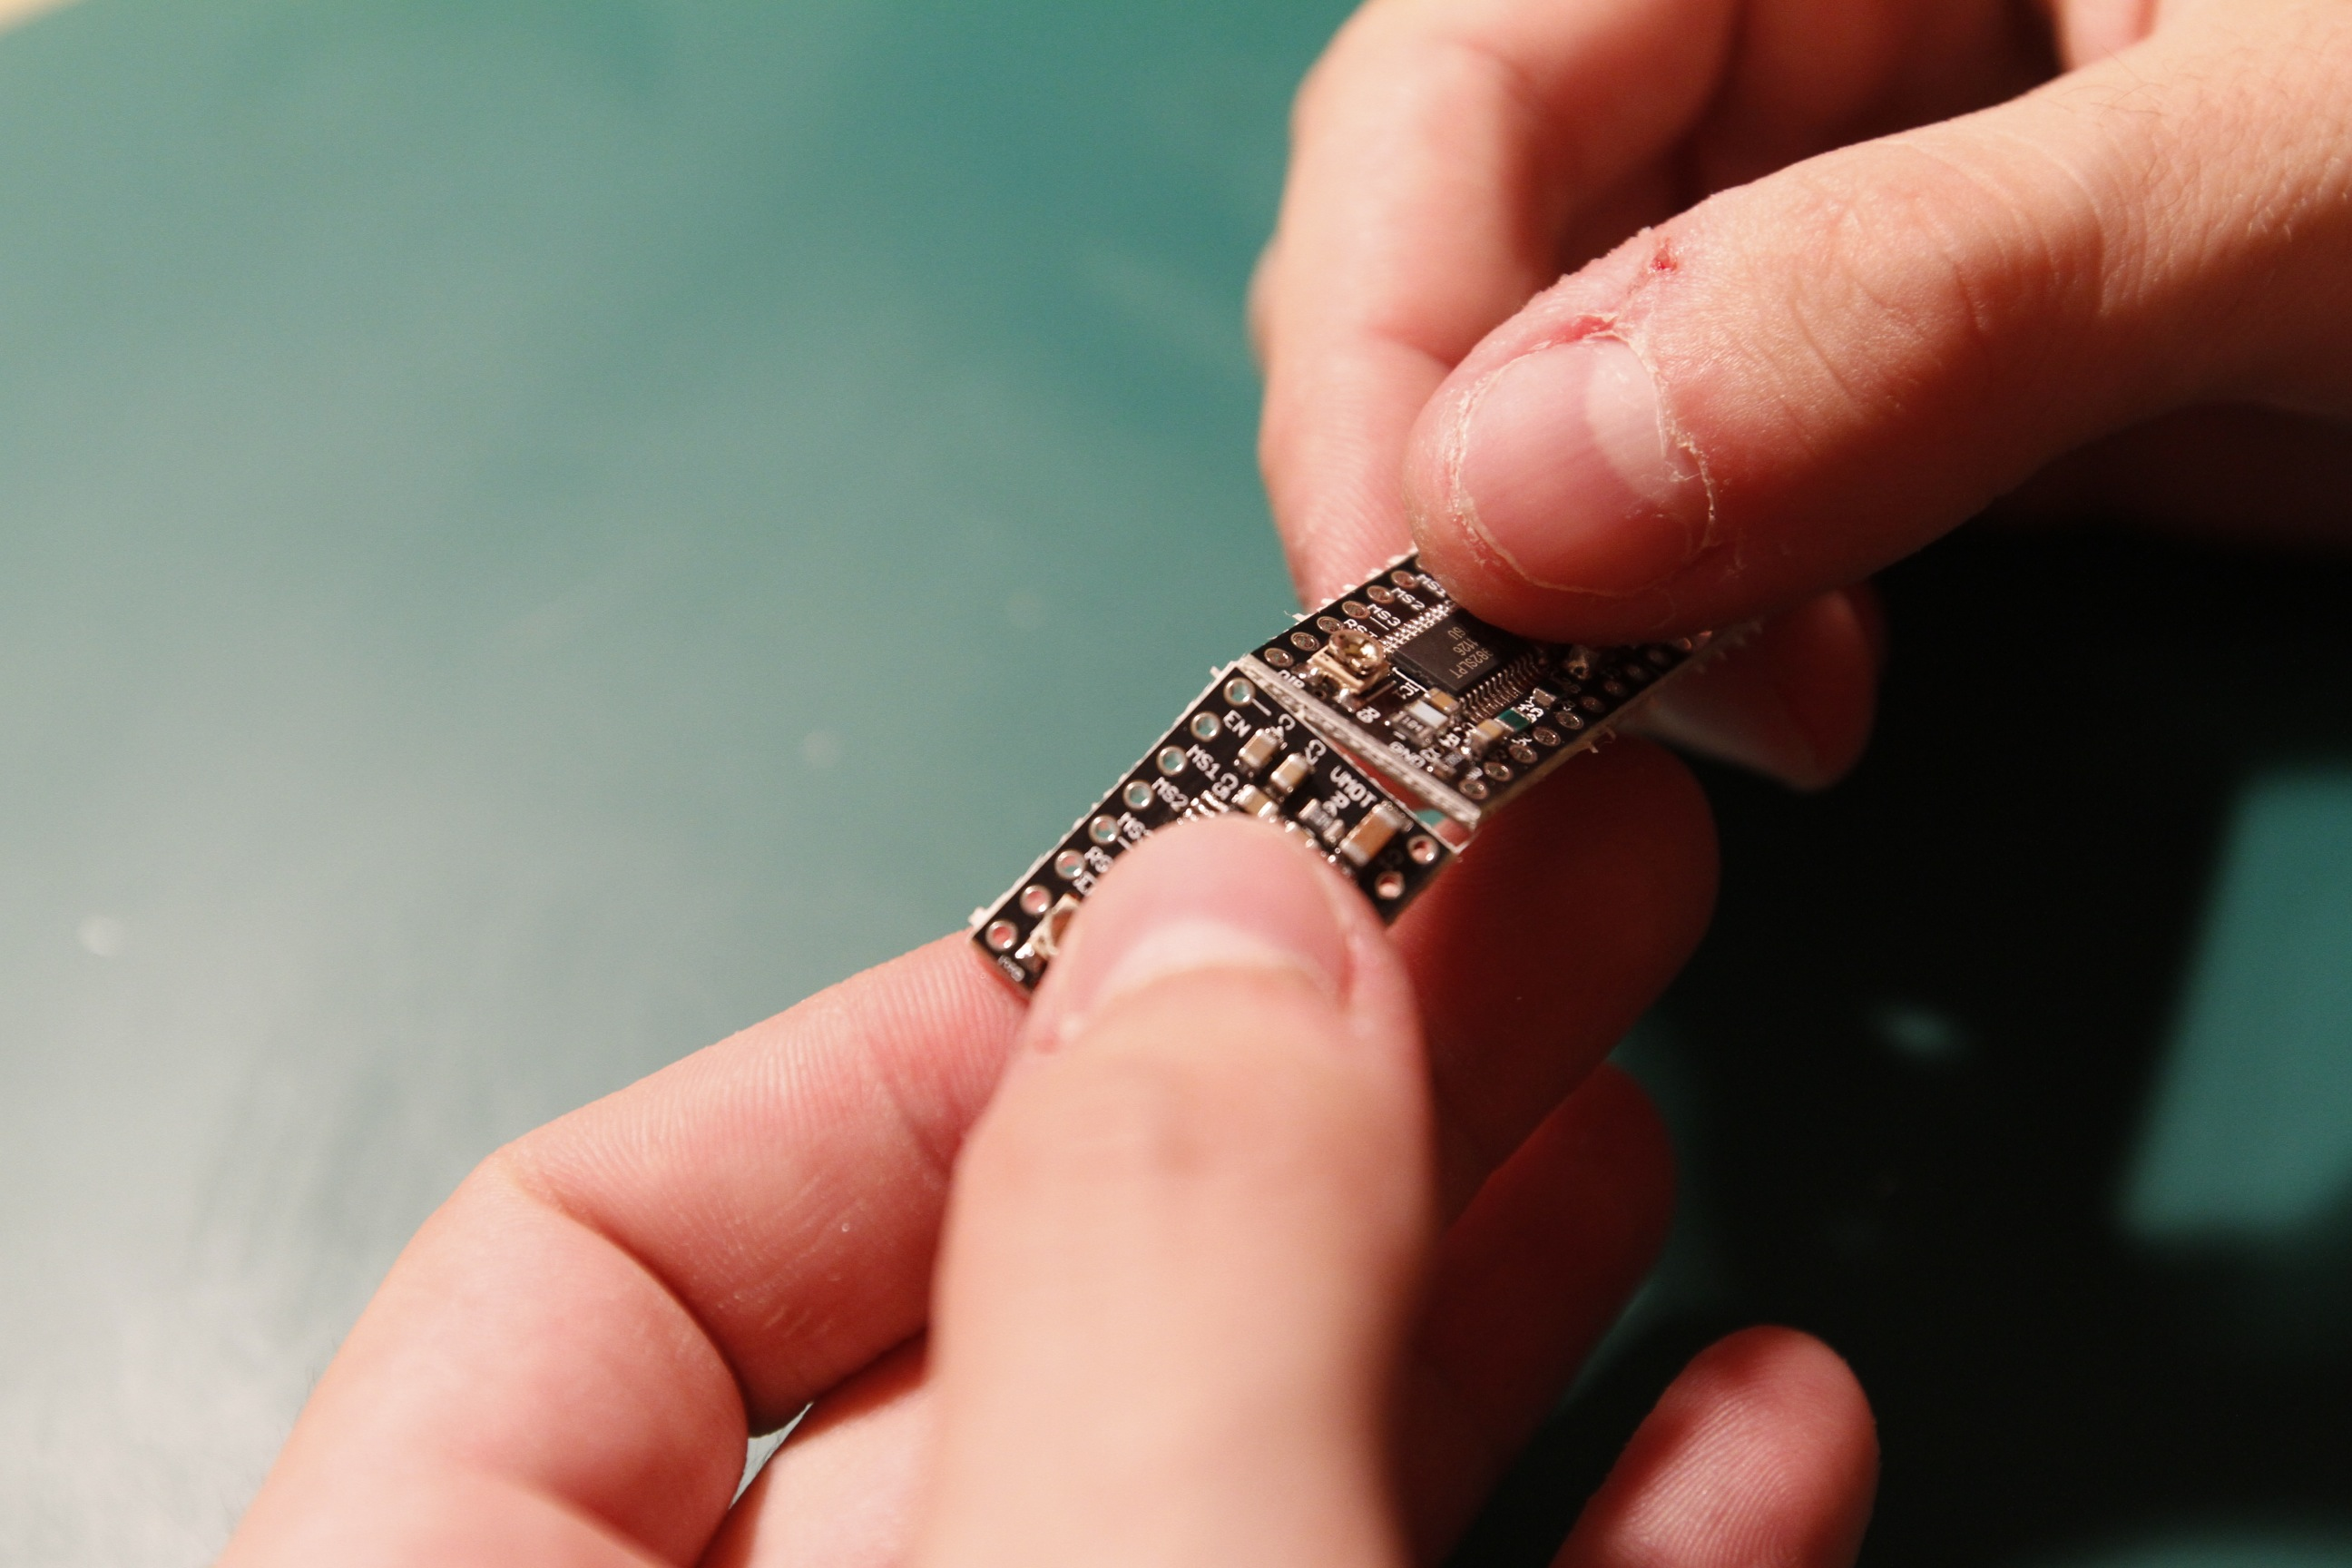
\includegraphics[width=0.7\textwidth]{../../Fotos/10.jpg}
				\caption{Separando los stepstick}
				\label{fig:cortar.stepstick}
			\end {figure}
				\begin{figure}[H]
				\centering
				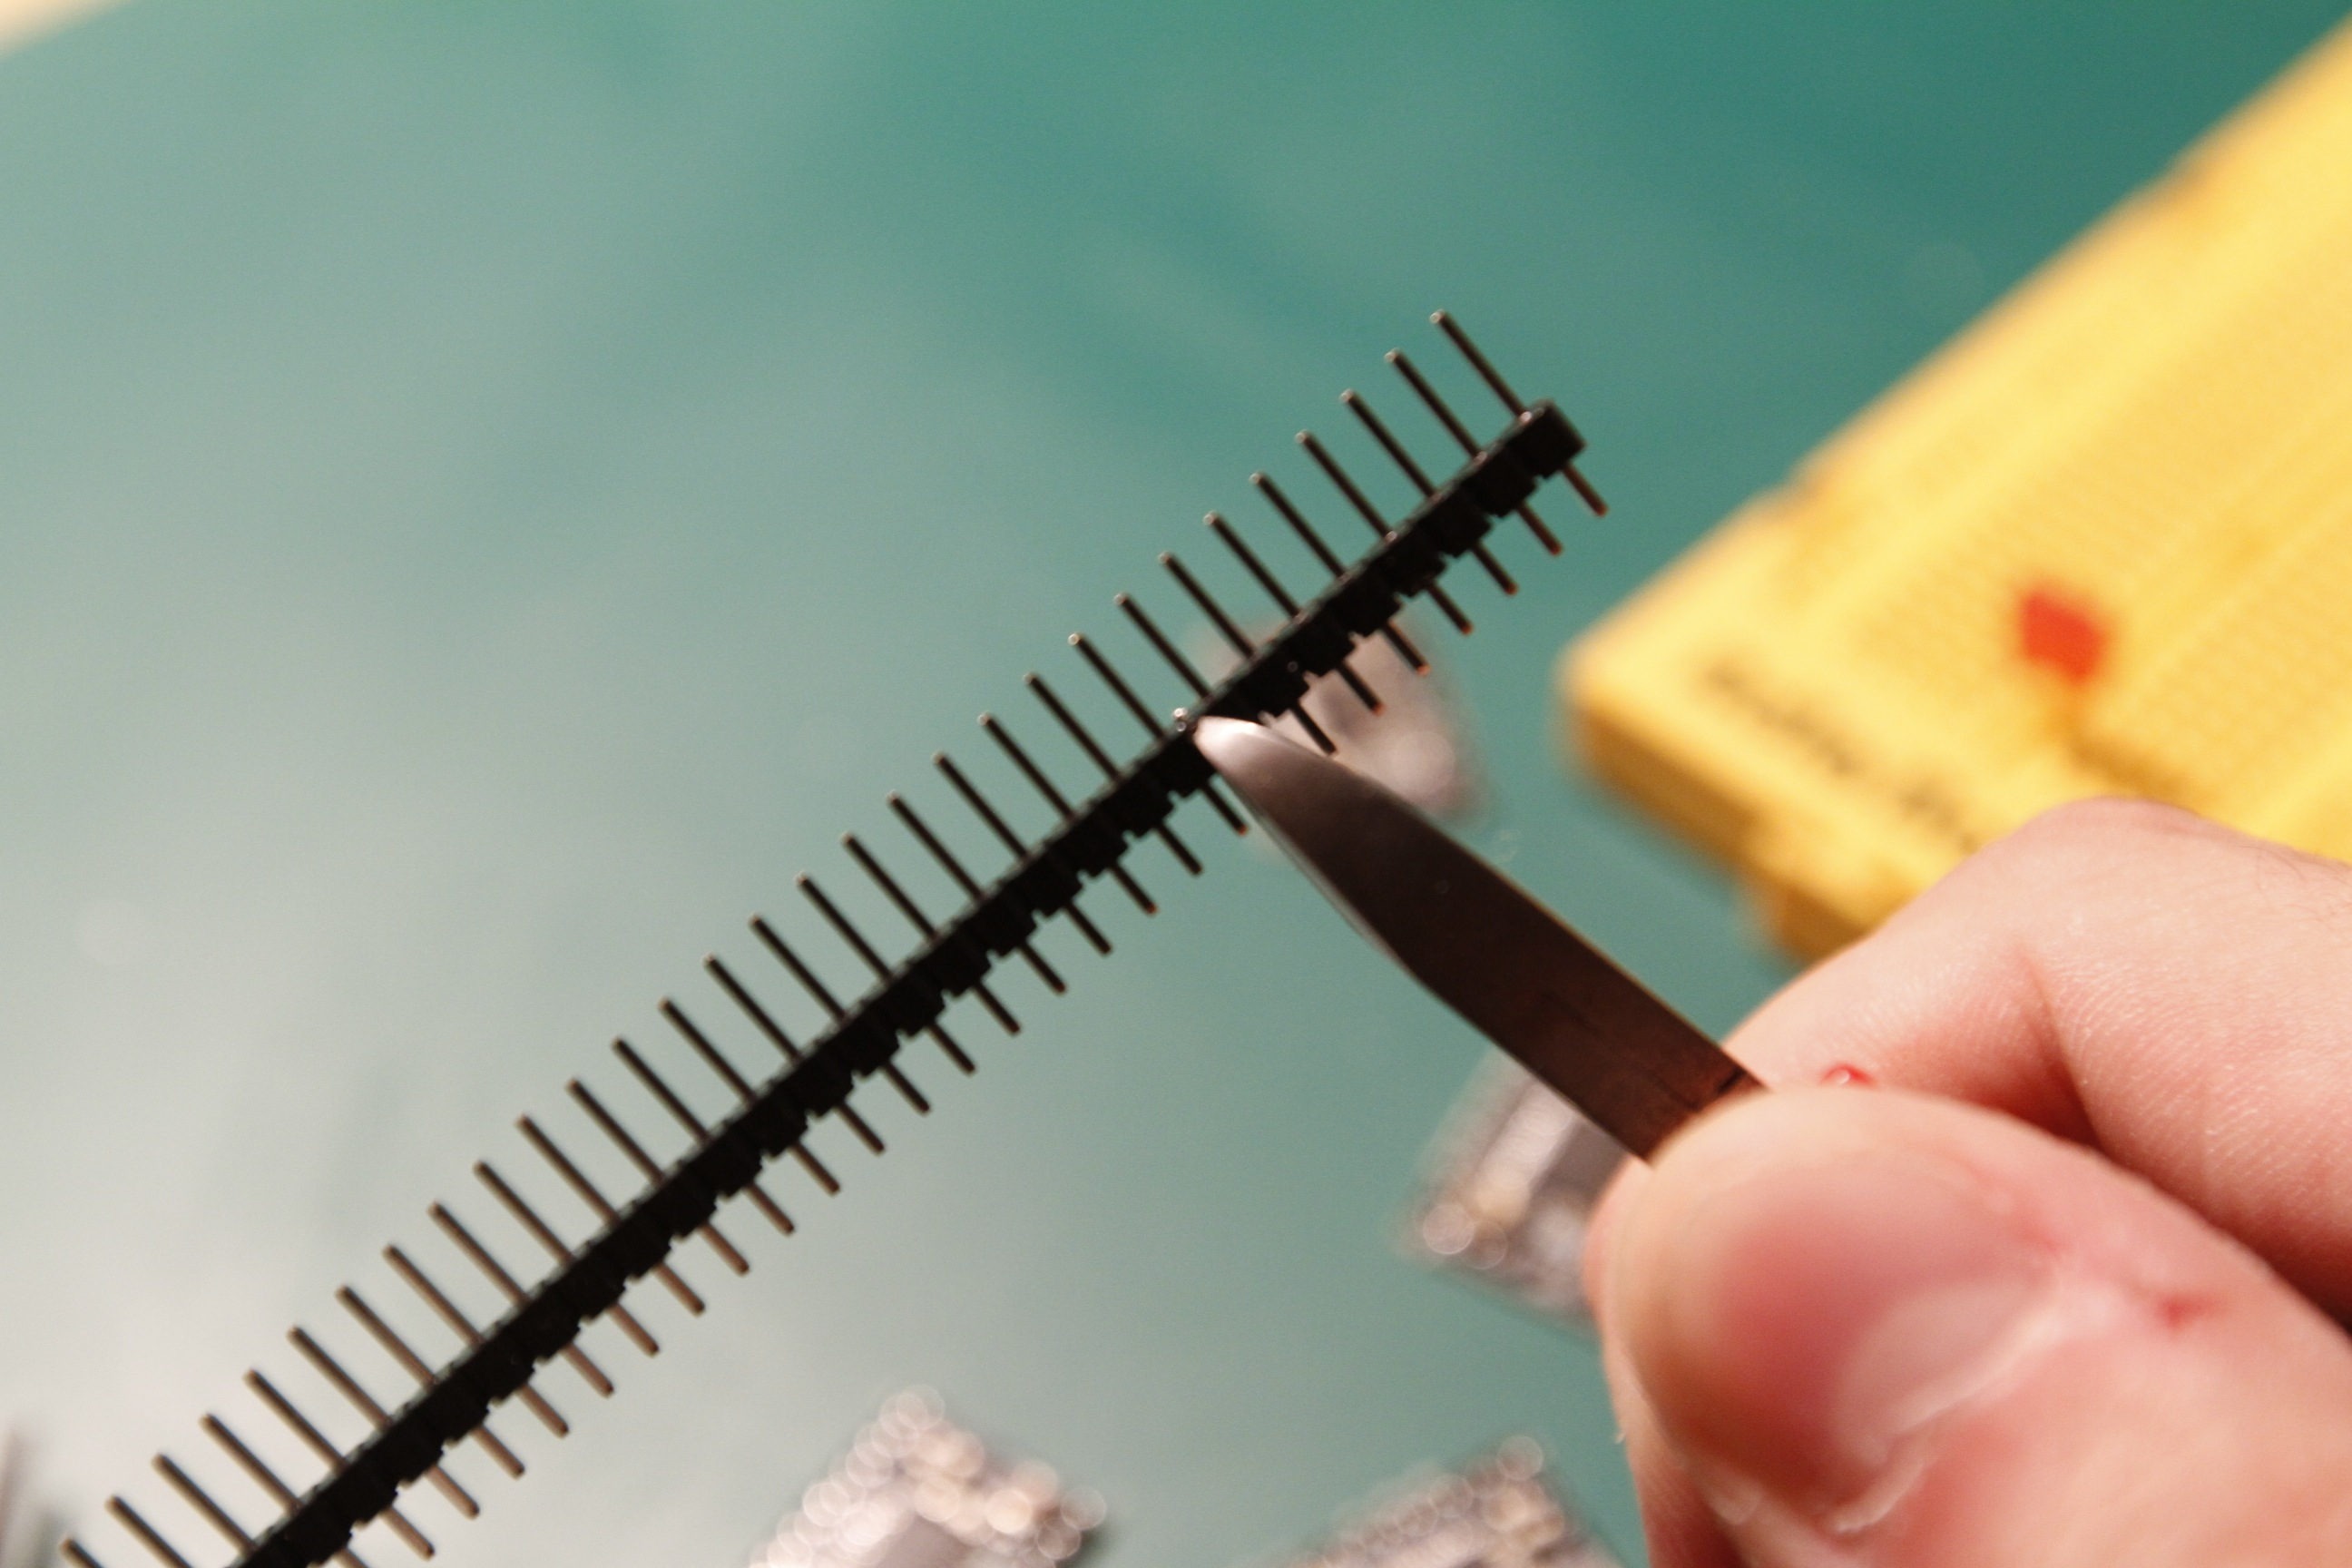
\includegraphics[width=0.7\textwidth]{../../Fotos/11.jpg}
				\caption{Separando los pines de conexión}
				\label{fig:cortar.pines}
			\end {figure}
			Colocamos dos filas de pines de 8 en el zocalo de la sanguinololu sin apretar y colocamos un driver de potencia como se muestra en la figura ~\ref{fig:zocalo.stepstick}. Una vez así colocado, soldamos los 4 pines de los extremos asegurandonos, de que el chip queda completamente pegado a los pins de forma horizontal. 
				\begin{figure}[H]
				\centering
				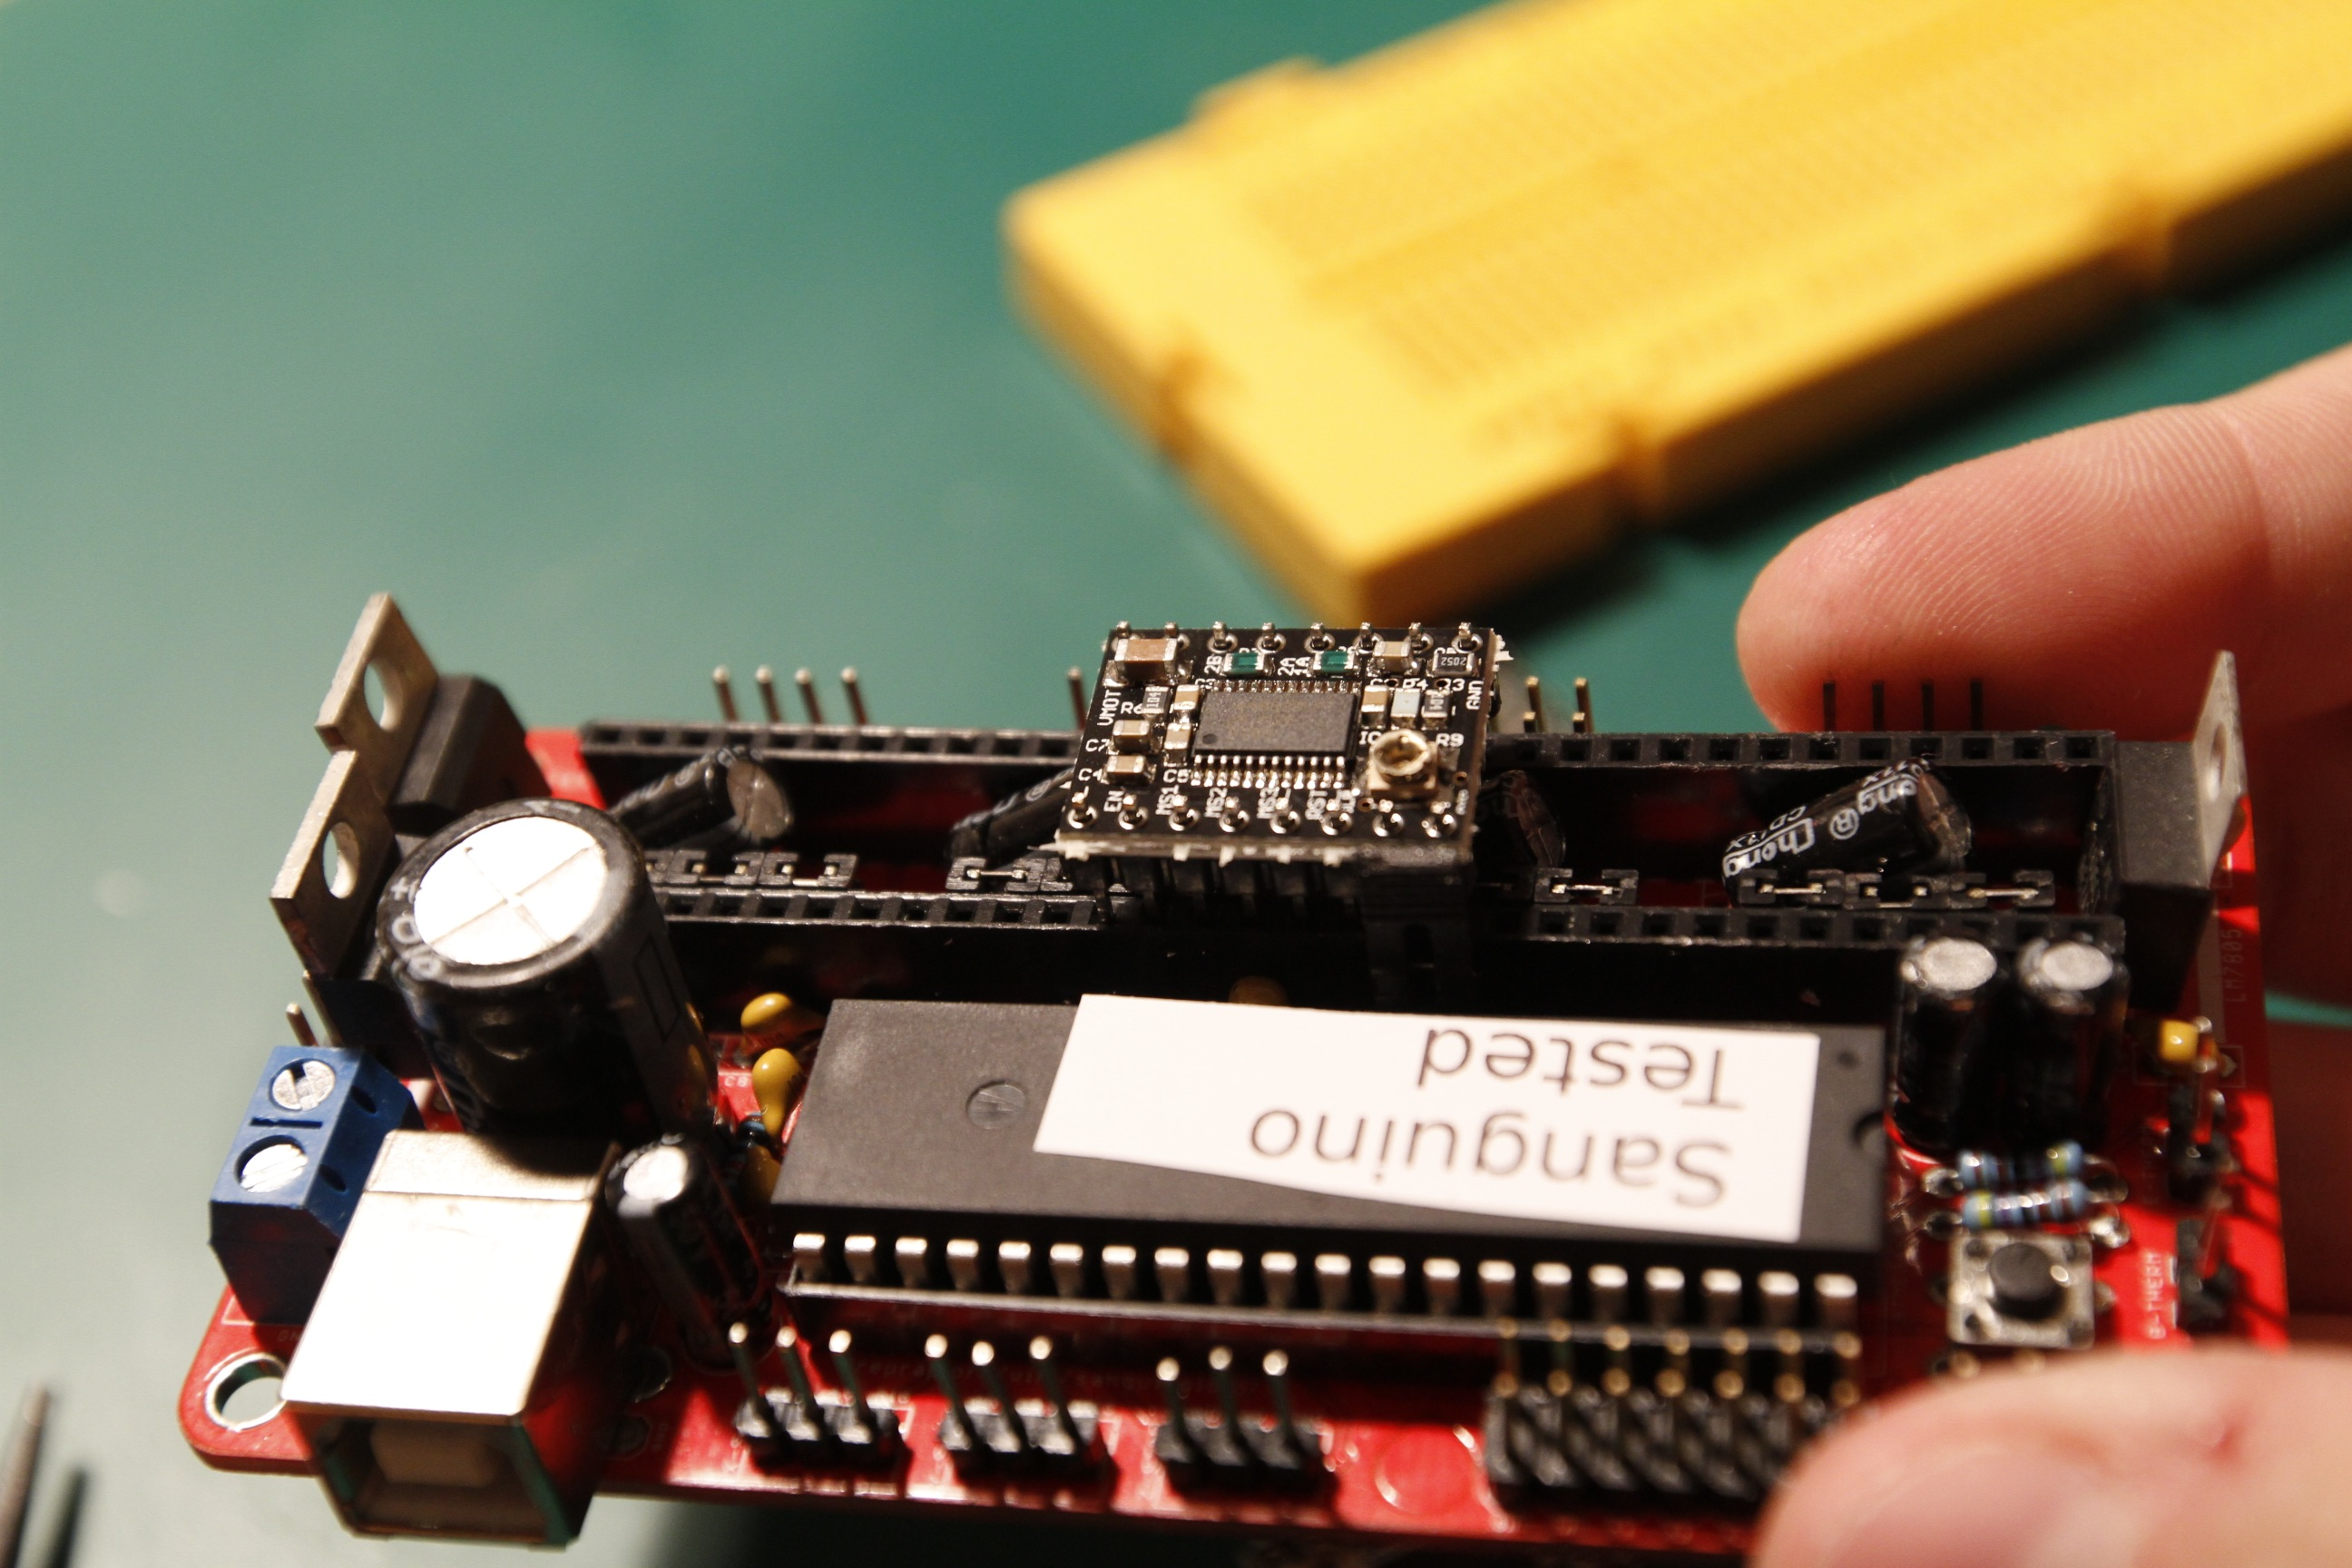
\includegraphics[width=0.7\textwidth]{../../Fotos/13.jpg}
				\caption{Colocando drivers de potencia}
				\label{fig:zocalo.stepstick}
			\end {figure}
			Quitamos el driver de la sanguinololu y soldamos de forma cómoda los pines que nos faltan. Al terminar, pasamos una lija de grano fino por los laterales del driver para dejar completamente liso la placa y que entre bien en la sanguinololu (Figura ~\ref{fig:limando.stepstick})
				\begin{figure}[H]
				\centering
				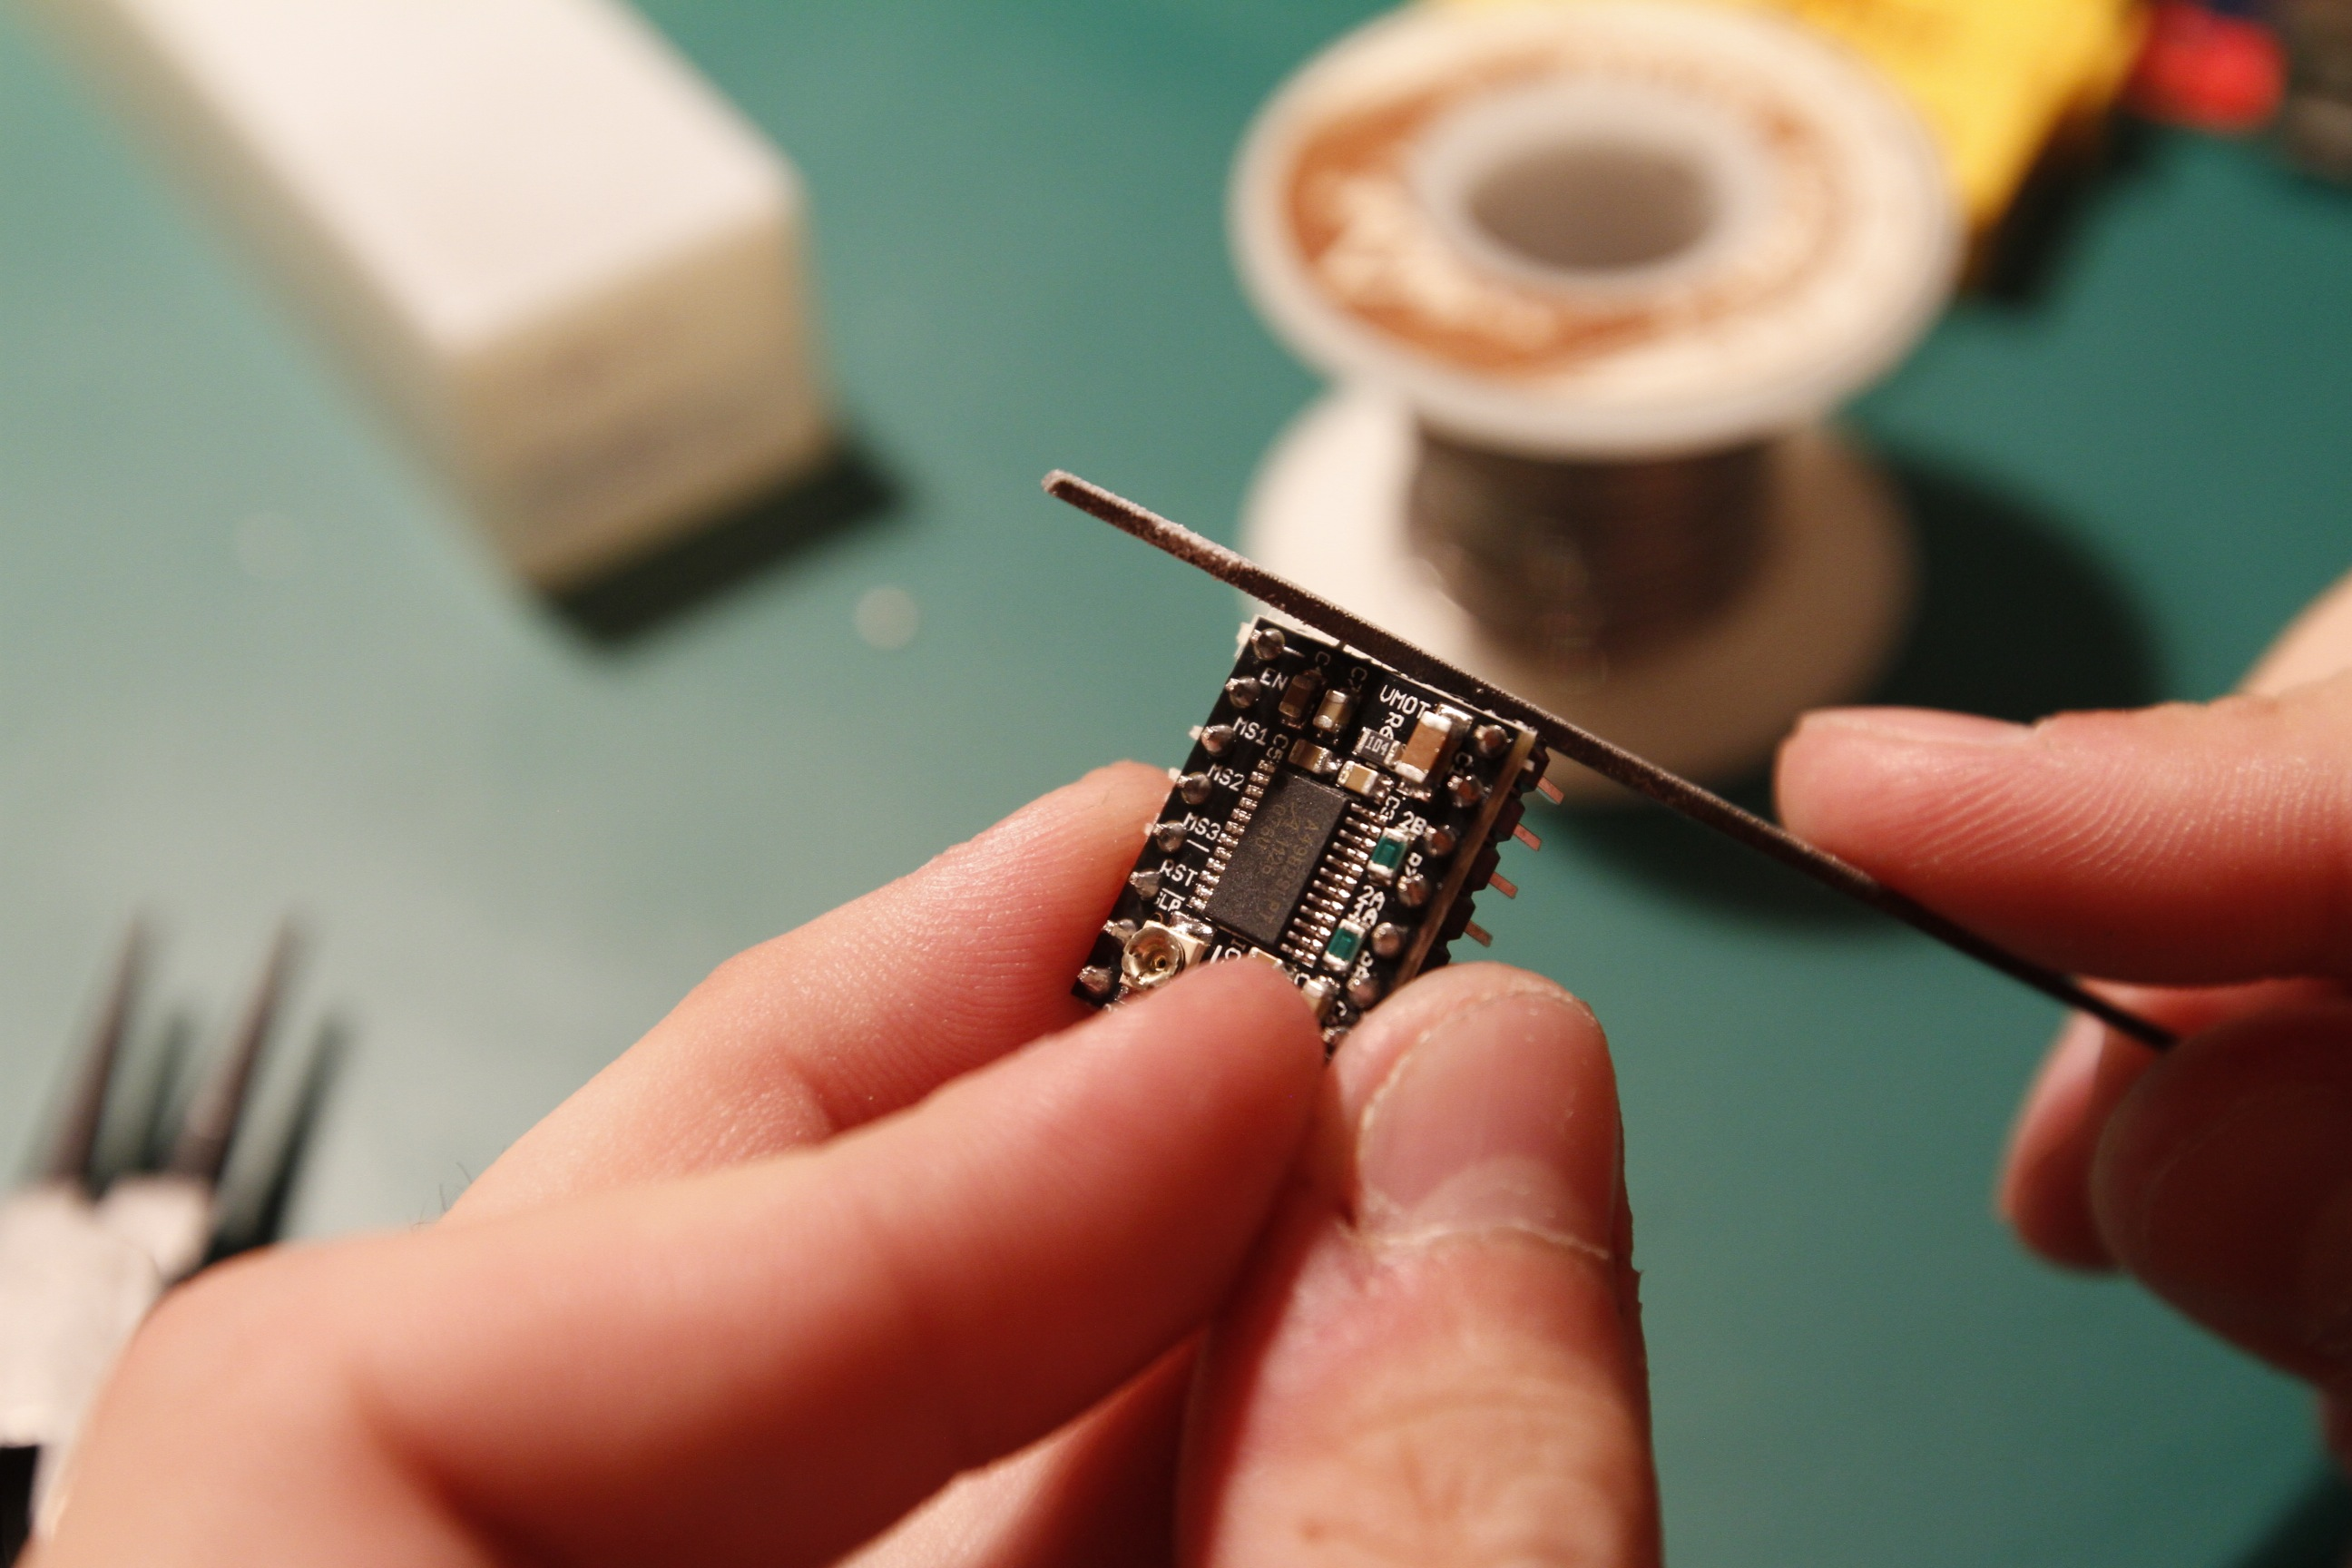
\includegraphics[width=0.7\textwidth]{../../Fotos/16.jpg}
				\caption{Limando drivers de potencia}
				\label{fig:limando.stepstick}
			\end {figure}
			Repetimos estos pasos con los 3 drivers y los colocamos de forma correcta en la placa. Es muy importante fijarse en la figura ~\ref{fig:colocando.stepstick} y ver como están colocados los drivers guiándonos por el potenciometro
				\begin{figure}[H]
				\centering
				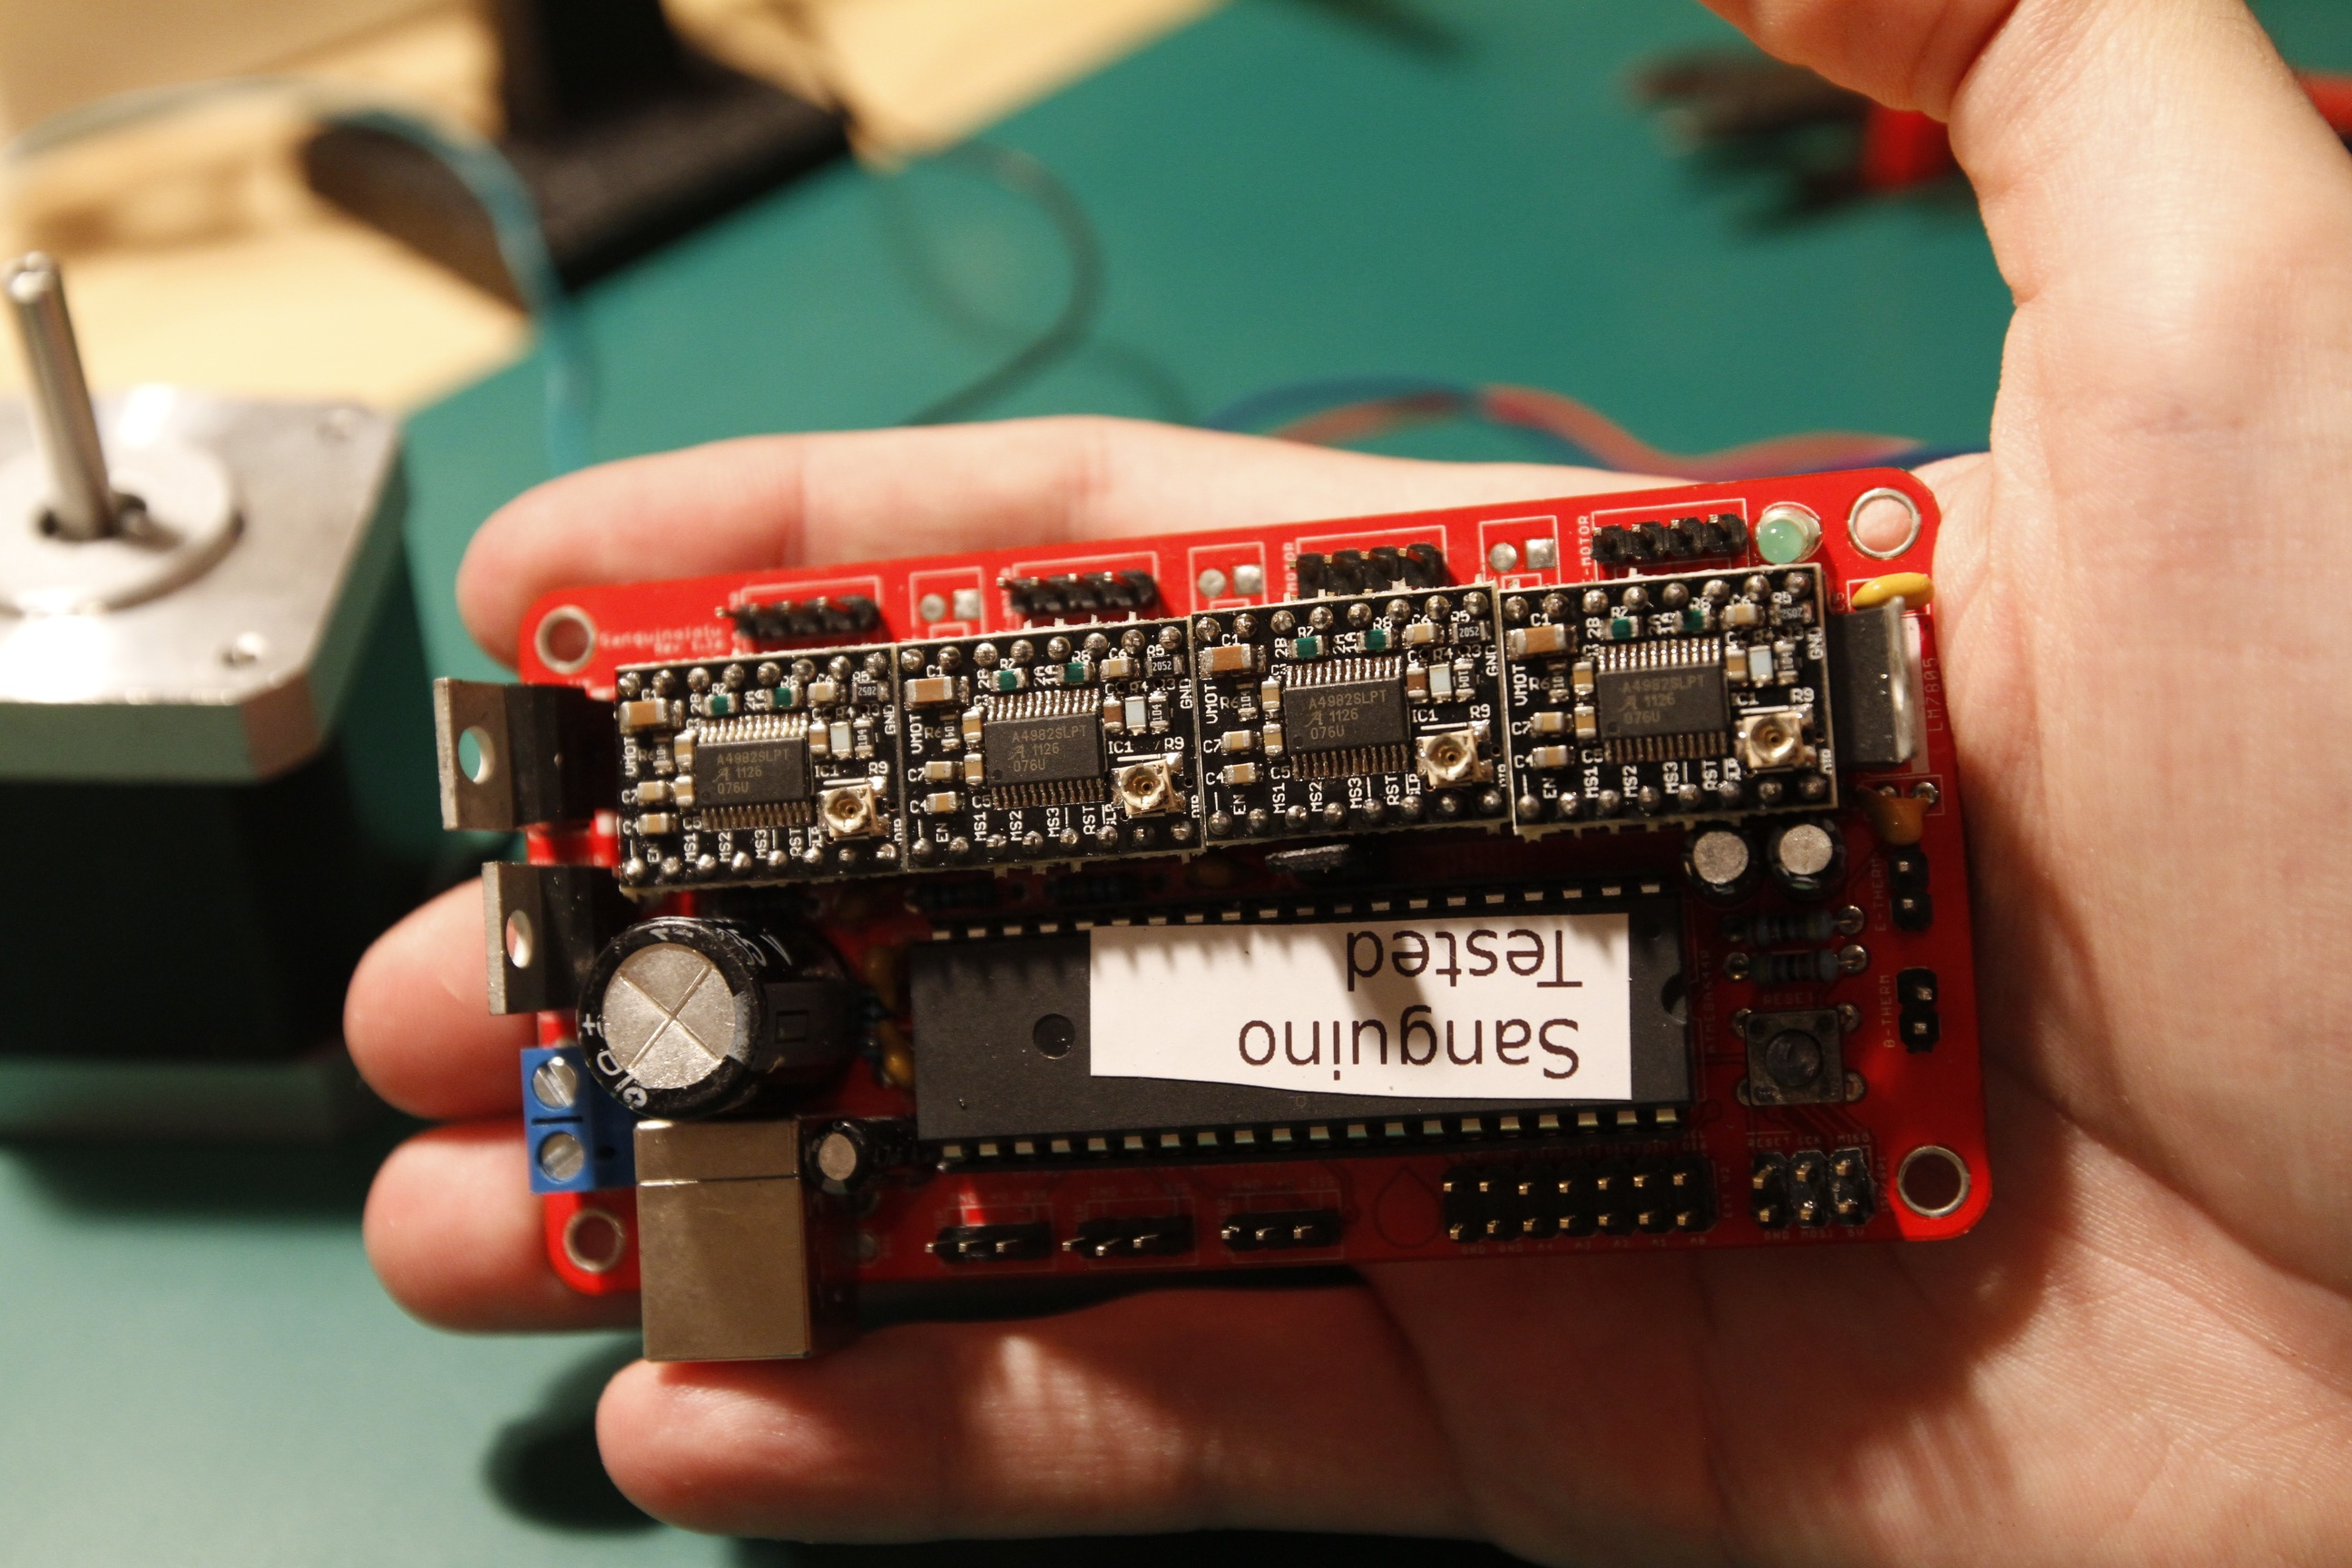
\includegraphics[width=0.7\textwidth]{../../Fotos/17.jpg}
				\caption{Sanguinololu con drivers de potencia}
				\label{fig:colocando.stepstick}
			\end {figure}
		\subsubsection{Preparando motores paso a paso}
		Los motores paso a paso tienen cuatro cables, cada dos de ellos van a una bobina; de este modo según vayamos mandando una señal a cada cable, el motor irá girando. Es necesario identificar a qué bobina va cada cable. Para ello basta con ir uniendo dos cables entre sí y girar el vástago del motor(Ver figura ~\ref{fig:cable.bobina}), si no conseguimos que se mueva esos dos cables irán juntos. Otra forma es poner un led en los extremos de los dos cables y girar el vástago, si el led se ilumina, los dos cables irán juntos(Figura ~\ref{fig:led.bobina}).\\

				\begin{figure}[H]
				        \centering
				        \begin{subfigure}[b]{0.4\textwidth}
				                \centering
				                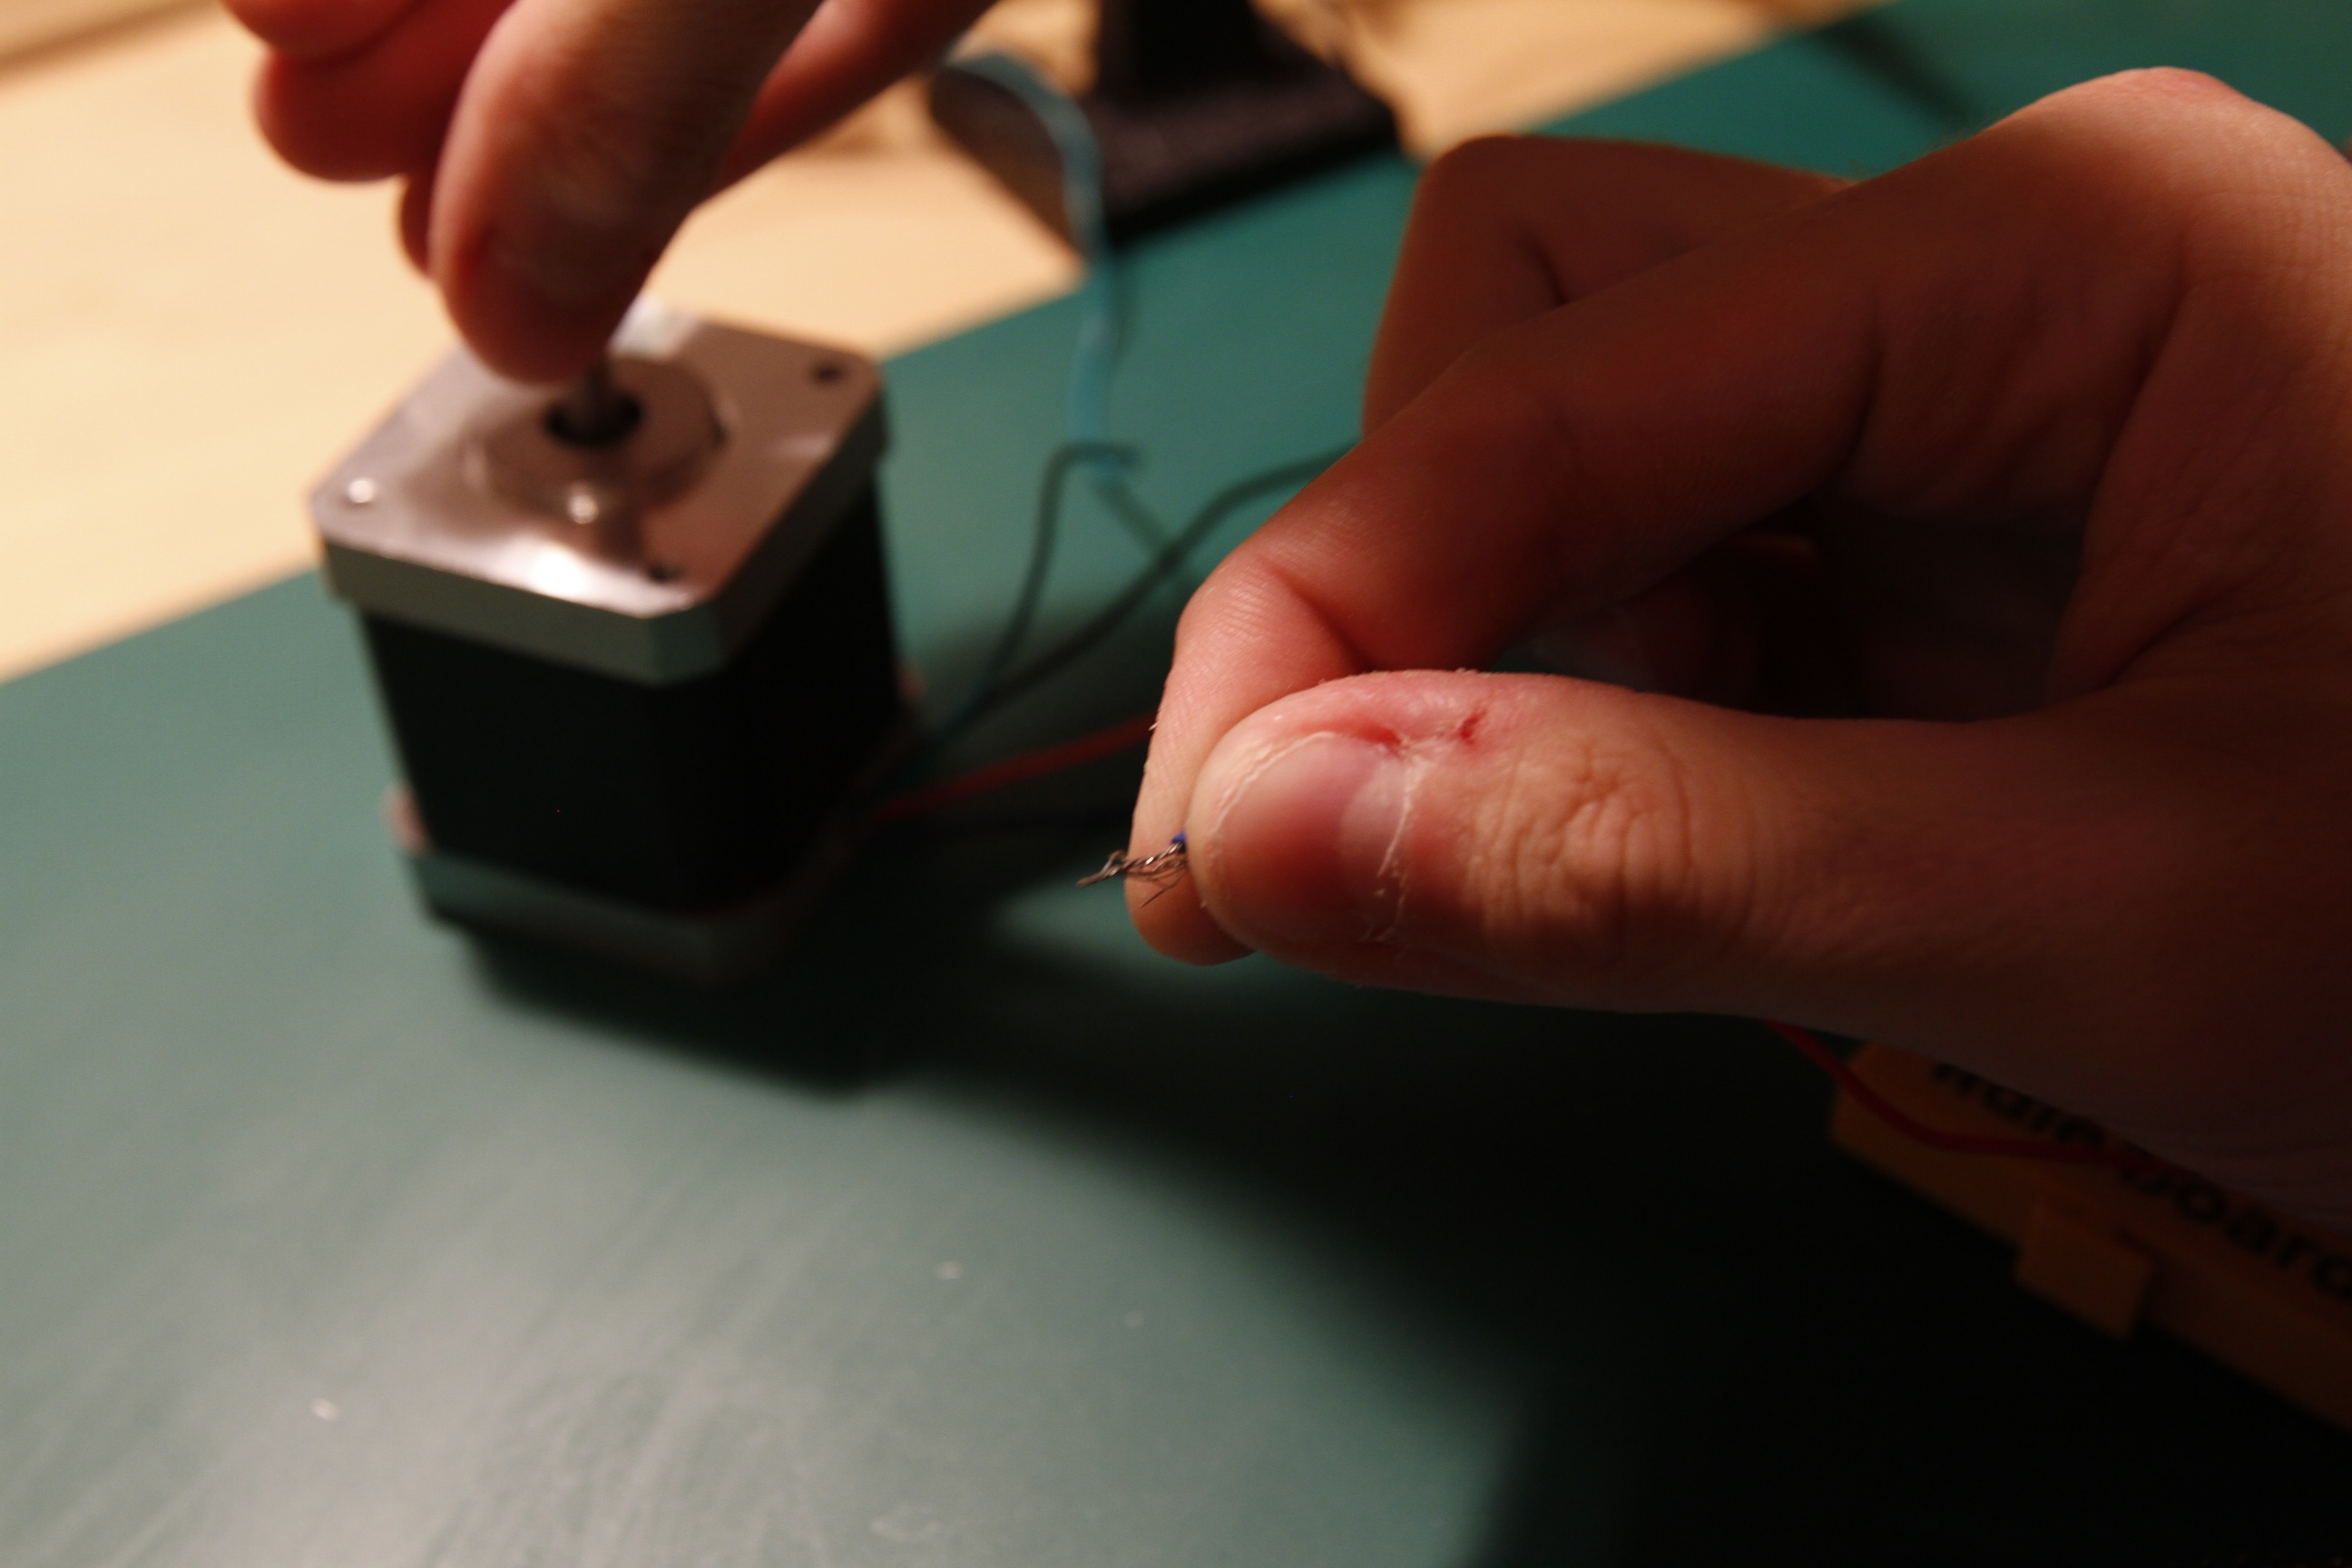
\includegraphics[width=\textwidth]{../../Fotos/19.jpg}
				                \caption{Uniendo cables }
				                \label{fig:cable.bobina}
				        \end{subfigure}
				        \begin{subfigure}[b]{0.4\textwidth}
				                \centering
				                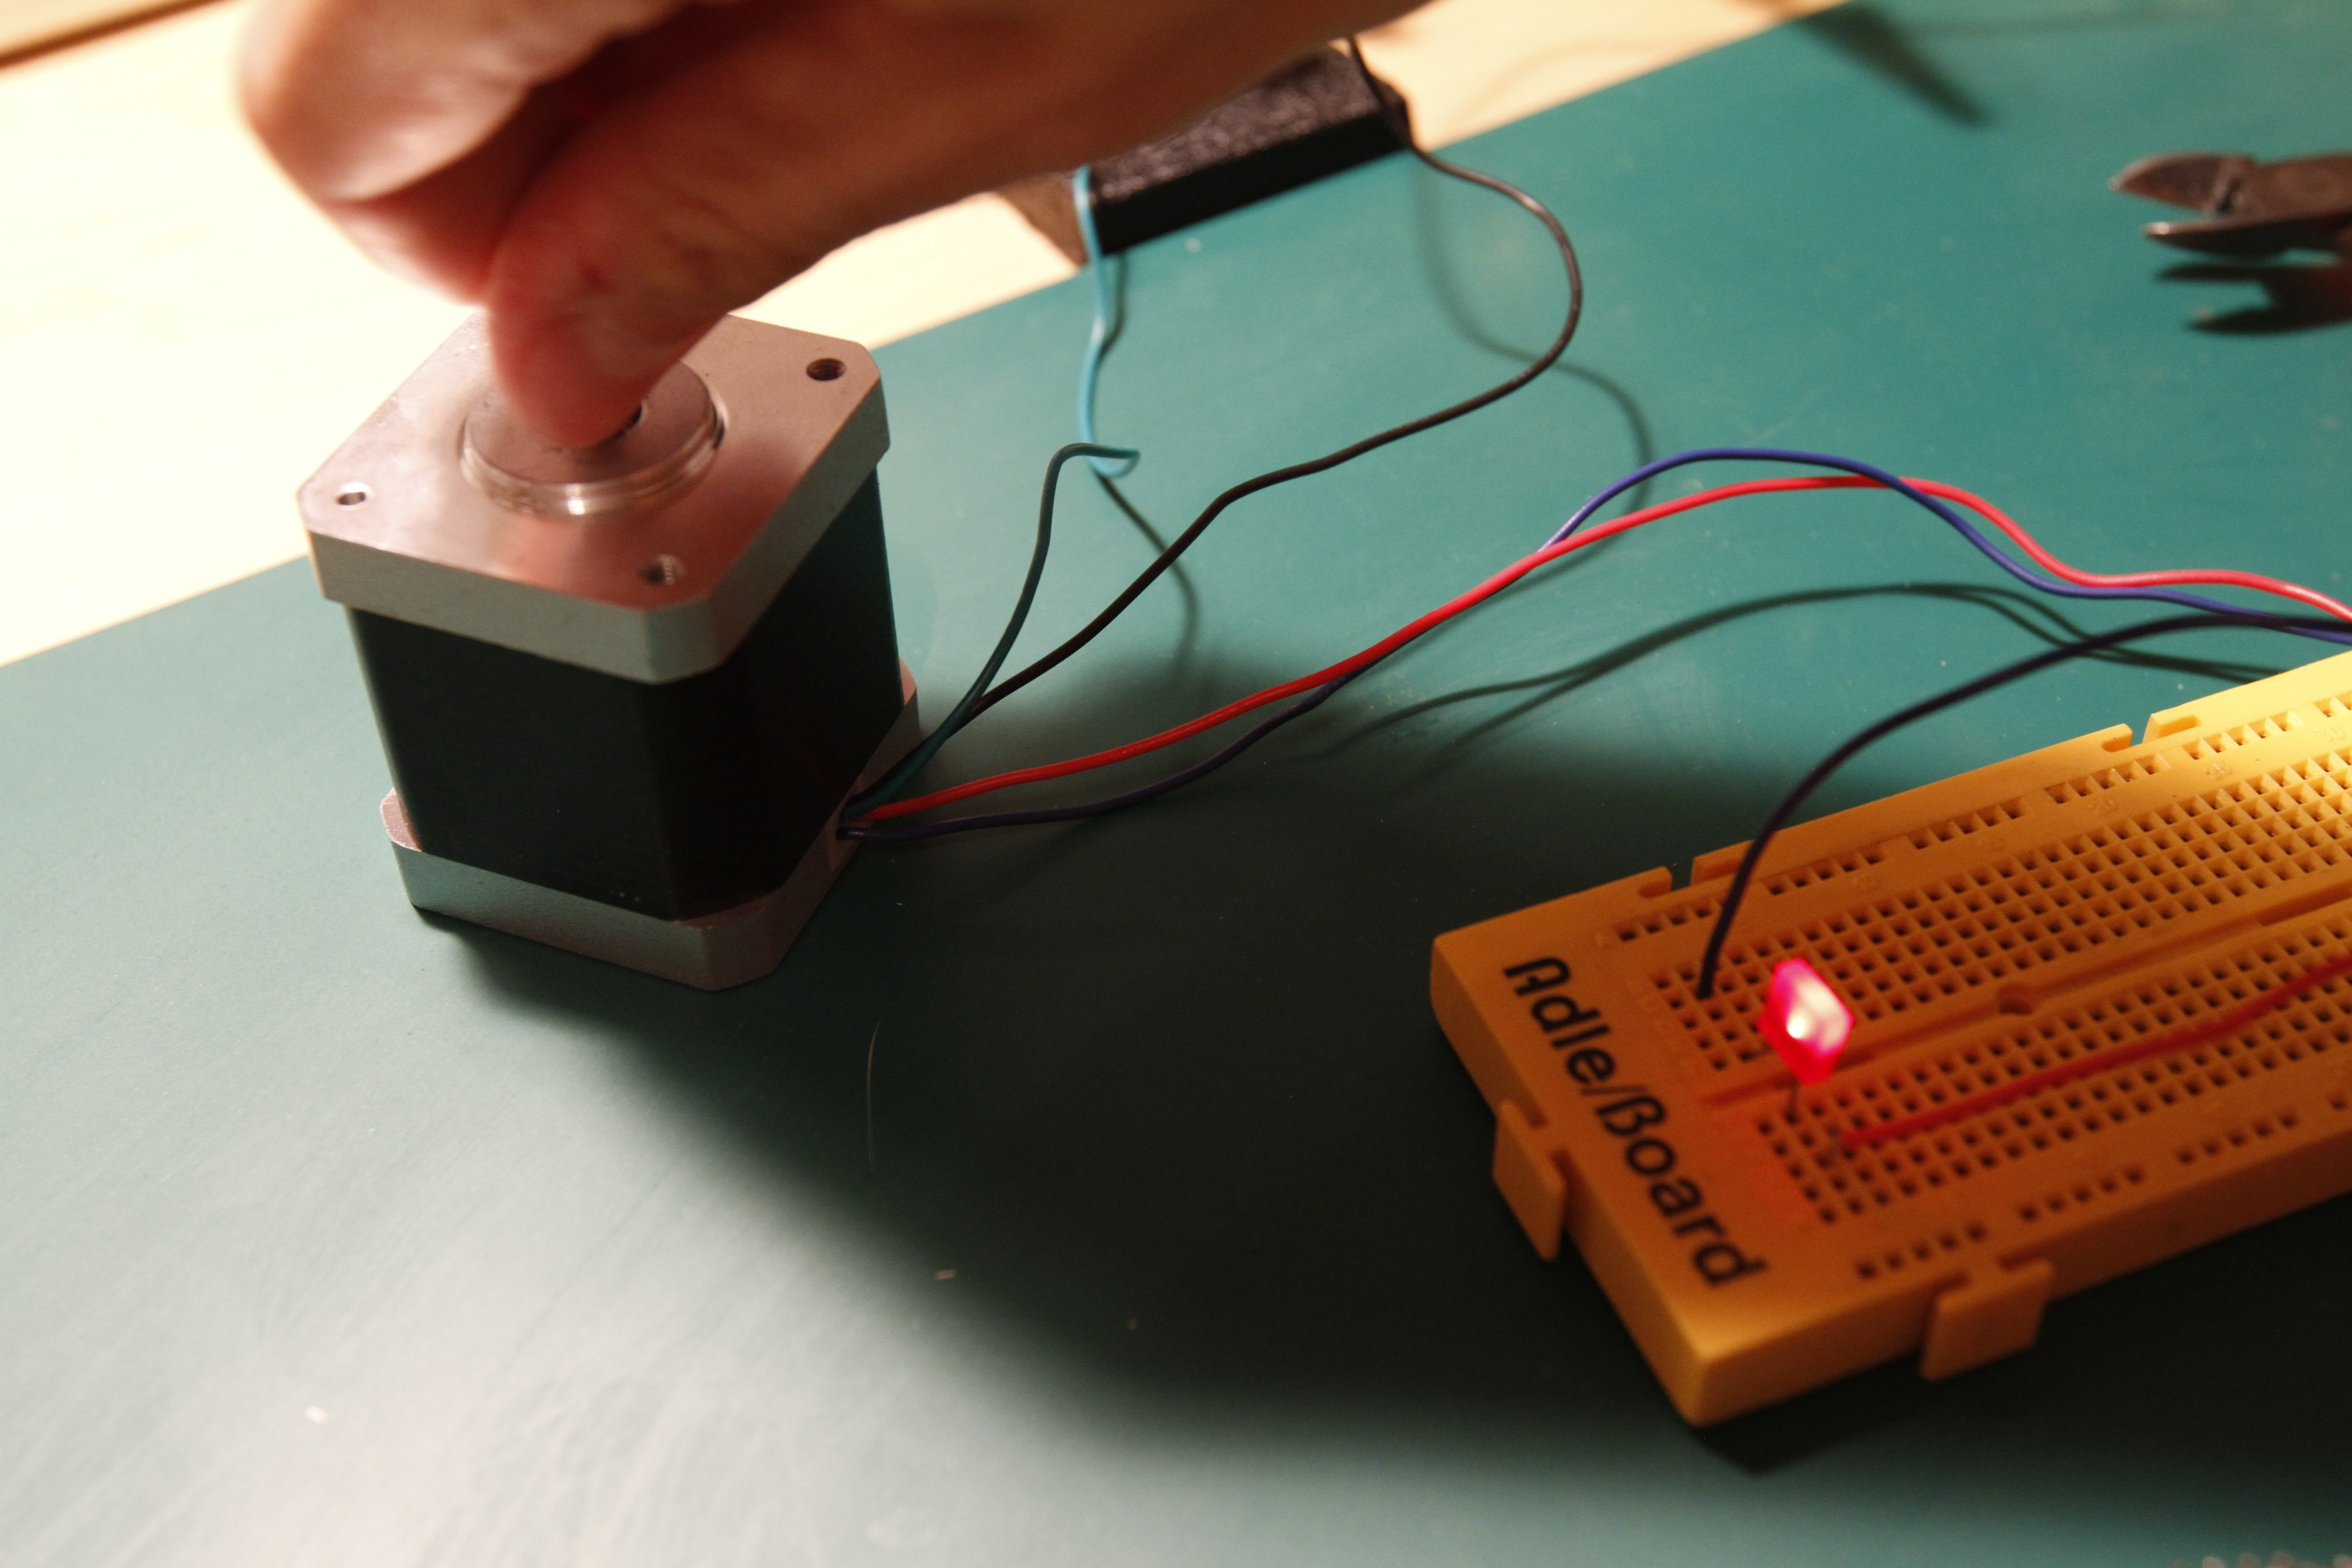
\includegraphics[width=\textwidth]{../../Fotos/18.jpg}
				                \caption{Mediante led}
				                \label{fig:led.bobina}
				        \end{subfigure}
				        \caption{Identificando bobinas paso a paso}\label{fig:bobinas}
				\end{figure}
				\newpage{}
				Una vez identificados los cables será necesario colocar primero los dos de una bobina seguidos de los otros cables de la bobina. \\
				\begin{table}[htb]
					\centering
				\begin{tabular}{|c|c|c|c|}
				\hline
				\multicolumn{2}{|c|}{Bobina 1} & \multicolumn{2}{|c|}{Bobina 2} \\
				\hline
					Rojo & Azul & Verde & Negro \\
				\hline
				\end{tabular}
				\caption{Código de colores de bobinas}
				\end{table}
				
		\subsubsection{Soldando end stop}
		Los endstop son los encargados de parar el motor cuando llegamos a uno de los extremos de la impresora. Se usan a la hora de hacer el home de la impresora y así indicarle que está en el origen de coordenadas. El otro extremo, para por software, indicamos el recorrido máximo y cuando el motor lo haya recorrido, no dejará avanzar más. El esquema que hay que seguir se puede ver en la figura ~\ref{fig:esquema.endstop}.
		\begin{figure}[H]
			\centering
			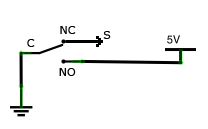
\includegraphics[width=0.7\textwidth]{../../Fotos/25.png}
			\caption{Esquema endstop}
			\label{fig:esquema.endstop}
		\end {figure}

		\subsubsection{Cargando firmware}
		Para cargar el firmware usaremos el software Arduino 023. A fecha de escribir el documento, la versión 1.0 da problemas. Y como firmware usaremos Marlin 1.0.\\
		Dentro del directorio de Marlin, veremos una carpeta que se llama \textbf{Sanguino}, la copiamos, y la llevamos dentro de nuestro Sketchbox a la carpeta \textbf{hardware}.En caso de no tener ninguna carpeta llamada harwdware, la creamos. Para ver cual es nuestra carpeta de Sketchbox abrimos arduino y nos vamos a las preferencias ~\ref{fig:pref.arduino}. Finalmente nos debería quedar algo parecido a lo que se muestra en la figura ~\ref{fig:sketchbox.arduino}\\
		Para evitar futuros problemas a la hora de cargar el firmare modificamos el fichero emph{boards.txt}, situado en el directorio sanguino, que acabamos de copiar .
		Cambiamos la linea en la que pone \emph{atmega644.upload.speed=57600} a \emph{atmega644.upload.speed=38400}.De este modo la carga será mucho más lenta, pero nos evitamos problemas de sincronización con la placa.\\
		
		\begin{figure}[H]
		        \centering
		        \begin{subfigure}[b]{0.7\textwidth}
		                \centering
		                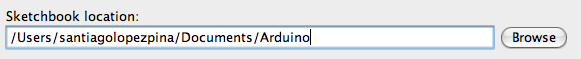
\includegraphics[width=\textwidth]{../../Fotos/29.png}
		                \caption{Preferencias de Arduino }
		                \label{fig:pref.arduino}
		        \end{subfigure}
		        \begin{subfigure}[b]{0.7\textwidth}
		                \centering
		                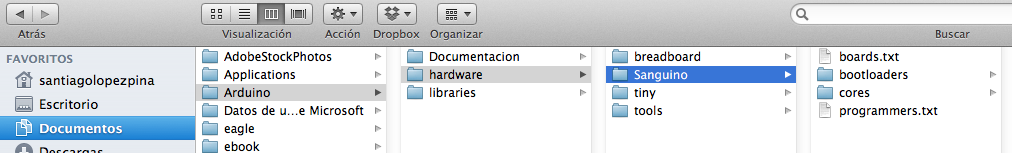
\includegraphics[width=\textwidth]{../../Fotos/30.png}
		                \caption{Sketchbox}
		                \label{fig:sketchbox.arduino}
		        \end{subfigure}
		        \caption{Configurando marlin}\label{fig:Marlin}
		\end{figure}
		Para comprobar que hemos hecho estos pasos bien, abrimos arduino y nos vamos a \emph{Tools>Board>Sanguino}. Si no nos aparece Sanguino deberemos cerciorarnos que hemos metido en el directorio correcto la carpeta \textbf{Sanguino} de Marlin.\\
		
		Una vez abierto marlin (fichero Marlin.pde), lo primero de todo es indicarle la placa que estamos usando, para ello nos vamos al fichero Configuration.h y en la linea 35 le indicamos qué versión de placa tenemos (Figura ~\ref{fig:sanguino.marlin})\\
		\begin{figure}[H]
			\centering
			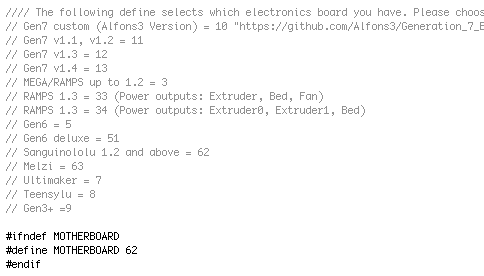
\includegraphics[width=0.7\textwidth]{../../Fotos/26.png}
			\caption{Configurando electrónica en marlin.}
			\label{fig:sanguino.marlin}
		\end {figure}
		Como inicialmente estaremos haciendo pruebas de los motores, es necesario indicar que de momento no usaremos ningún termistor, de este modo marlin nos dejará trabajar correctamente. Para ello en las lineas 64 y 67 pondremos 0.
		\begin{figure}[H]
			\centering
			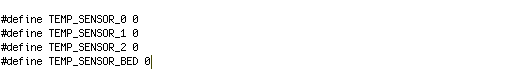
\includegraphics[width=0.7\textwidth]{../../Fotos/28.png}
			\caption{Configurando termistores en marlin.}
			\label{fig:termistor1.marlin}
		\end {figure}
A continuación le indicaremos como tenemos configurados los end-stop, si hemos seguido el esquemático indicado en la figura ~\ref{fig:esquema.endstop}, en la configuración de los endstop pondremos \textbf{\emph{false}} en las lineas 162,163 y 164.

		\begin{figure}[H]
			\centering
			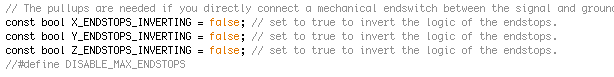
\includegraphics[width=0.7\textwidth]{../../Fotos/27.png}
			\caption{Configurando endstop en marlin.}
			\label{fig:endstop.marlin}
		\end {figure}
		Una de las mejoras que trae Marlin, es que añade aceleraciones a los motores paso a paso. Esto es puede ser una mejora, pero si tenemos un valor equivocado nos puede ocasionar pérdida de pasos, debido a que Marlin le pide una aceleración mayor a la que los motores físicamente puede. Para ello, nos vamos al fichero \emph{Configuration.h}, y buscamos la linea 220 las configuraciones de \textbf{DEFAULT MAX FEEDRATE} y \textbf{DEFAULT MAX ACCELERATION}. Ponemos los valores que vemos en la figura ~\ref{fig:aceleracions.marlin}\\
		\begin{figure}[H]
			\centering
			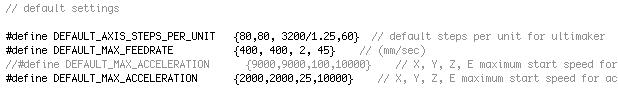
\includegraphics[width=0.7\textwidth]{../../Fotos/45.png}
			\caption{Configurando aceleraciones en Marlin.}
			\label{fig:aceleracions.marlin}
		\end {figure}
		Una vez hechas estás modificaciones, volvemos al fichero Marlin.pde, comprobamos que en \emph{Tools>Board>} tenemos elegido sanguino y en \emph{Tools>Serial Port>} está correctamente el usb y compilamos. Una vez terminado de compilar cargamos el programa. Es muy importante que tengamos puesto el jumper de Reset en la placa, viene puesto por defecto (Ver figura ~\ref{fig:jumper.sanguino}). Cargamos el programa a la placa y si no hay ningún problema debería finalizar correctamente.
		
		\begin{figure}[H]
			\centering
			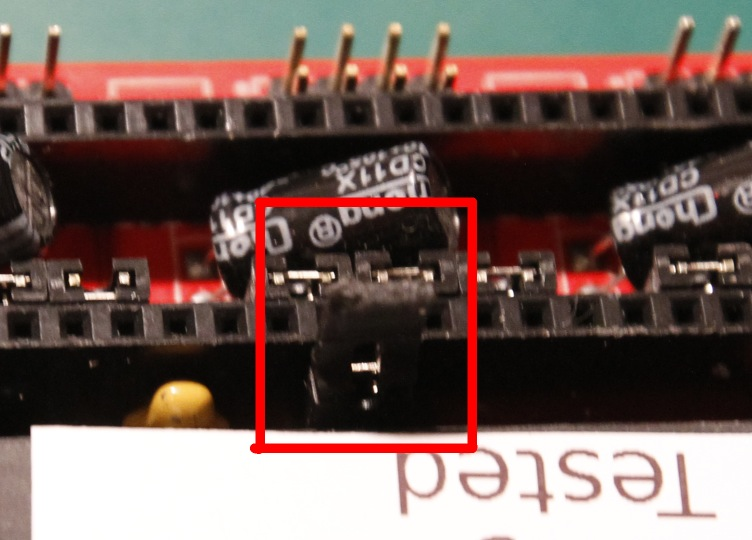
\includegraphics[width=0.7\textwidth]{../../Fotos/7.jpg}
			\caption{Jumper autoreset en sanguino.}
			\label{fig:jumper.sanguino}
		\end {figure}
		\newpage{}	
		\subsubsection{Ajustando intensidad drivers de potencia}
		Para esta parte nos hará falta tener al menos dos motores y un endstop cableados. Lo conectamos a la sanguinololu siguiendo el esquema oficial de Reprap (Ver figura ~\ref{fig:esquema.sanguino}).\\
		\begin{figure}[H]
			\centering
			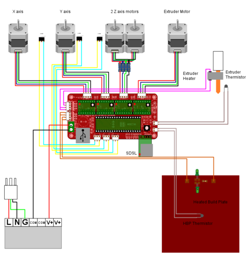
\includegraphics[width=0.5\textwidth]{../../Fotos/31.png}
			\caption{Esquemático sanguino.}
			\label{fig:esquema.sanguino}
		\end {figure}
Antes de continuar será necesario modificar la fuente de alimentación. Para ello, localizaremos el conector de 20 pines rectangular y juntaremos los cables verde y negro (Figura ~\ref{fig:atx.fuente}). Y uniremos dos cables amarillos y dos negros, cualesquiera mediante un punto de soldadura (Figura ~\ref{fig:vcc.fuente}).\\
			\begin{figure}[H]
			        \centering
			        \begin{subfigure}[htb]{0.4\textwidth}
			                \centering
			                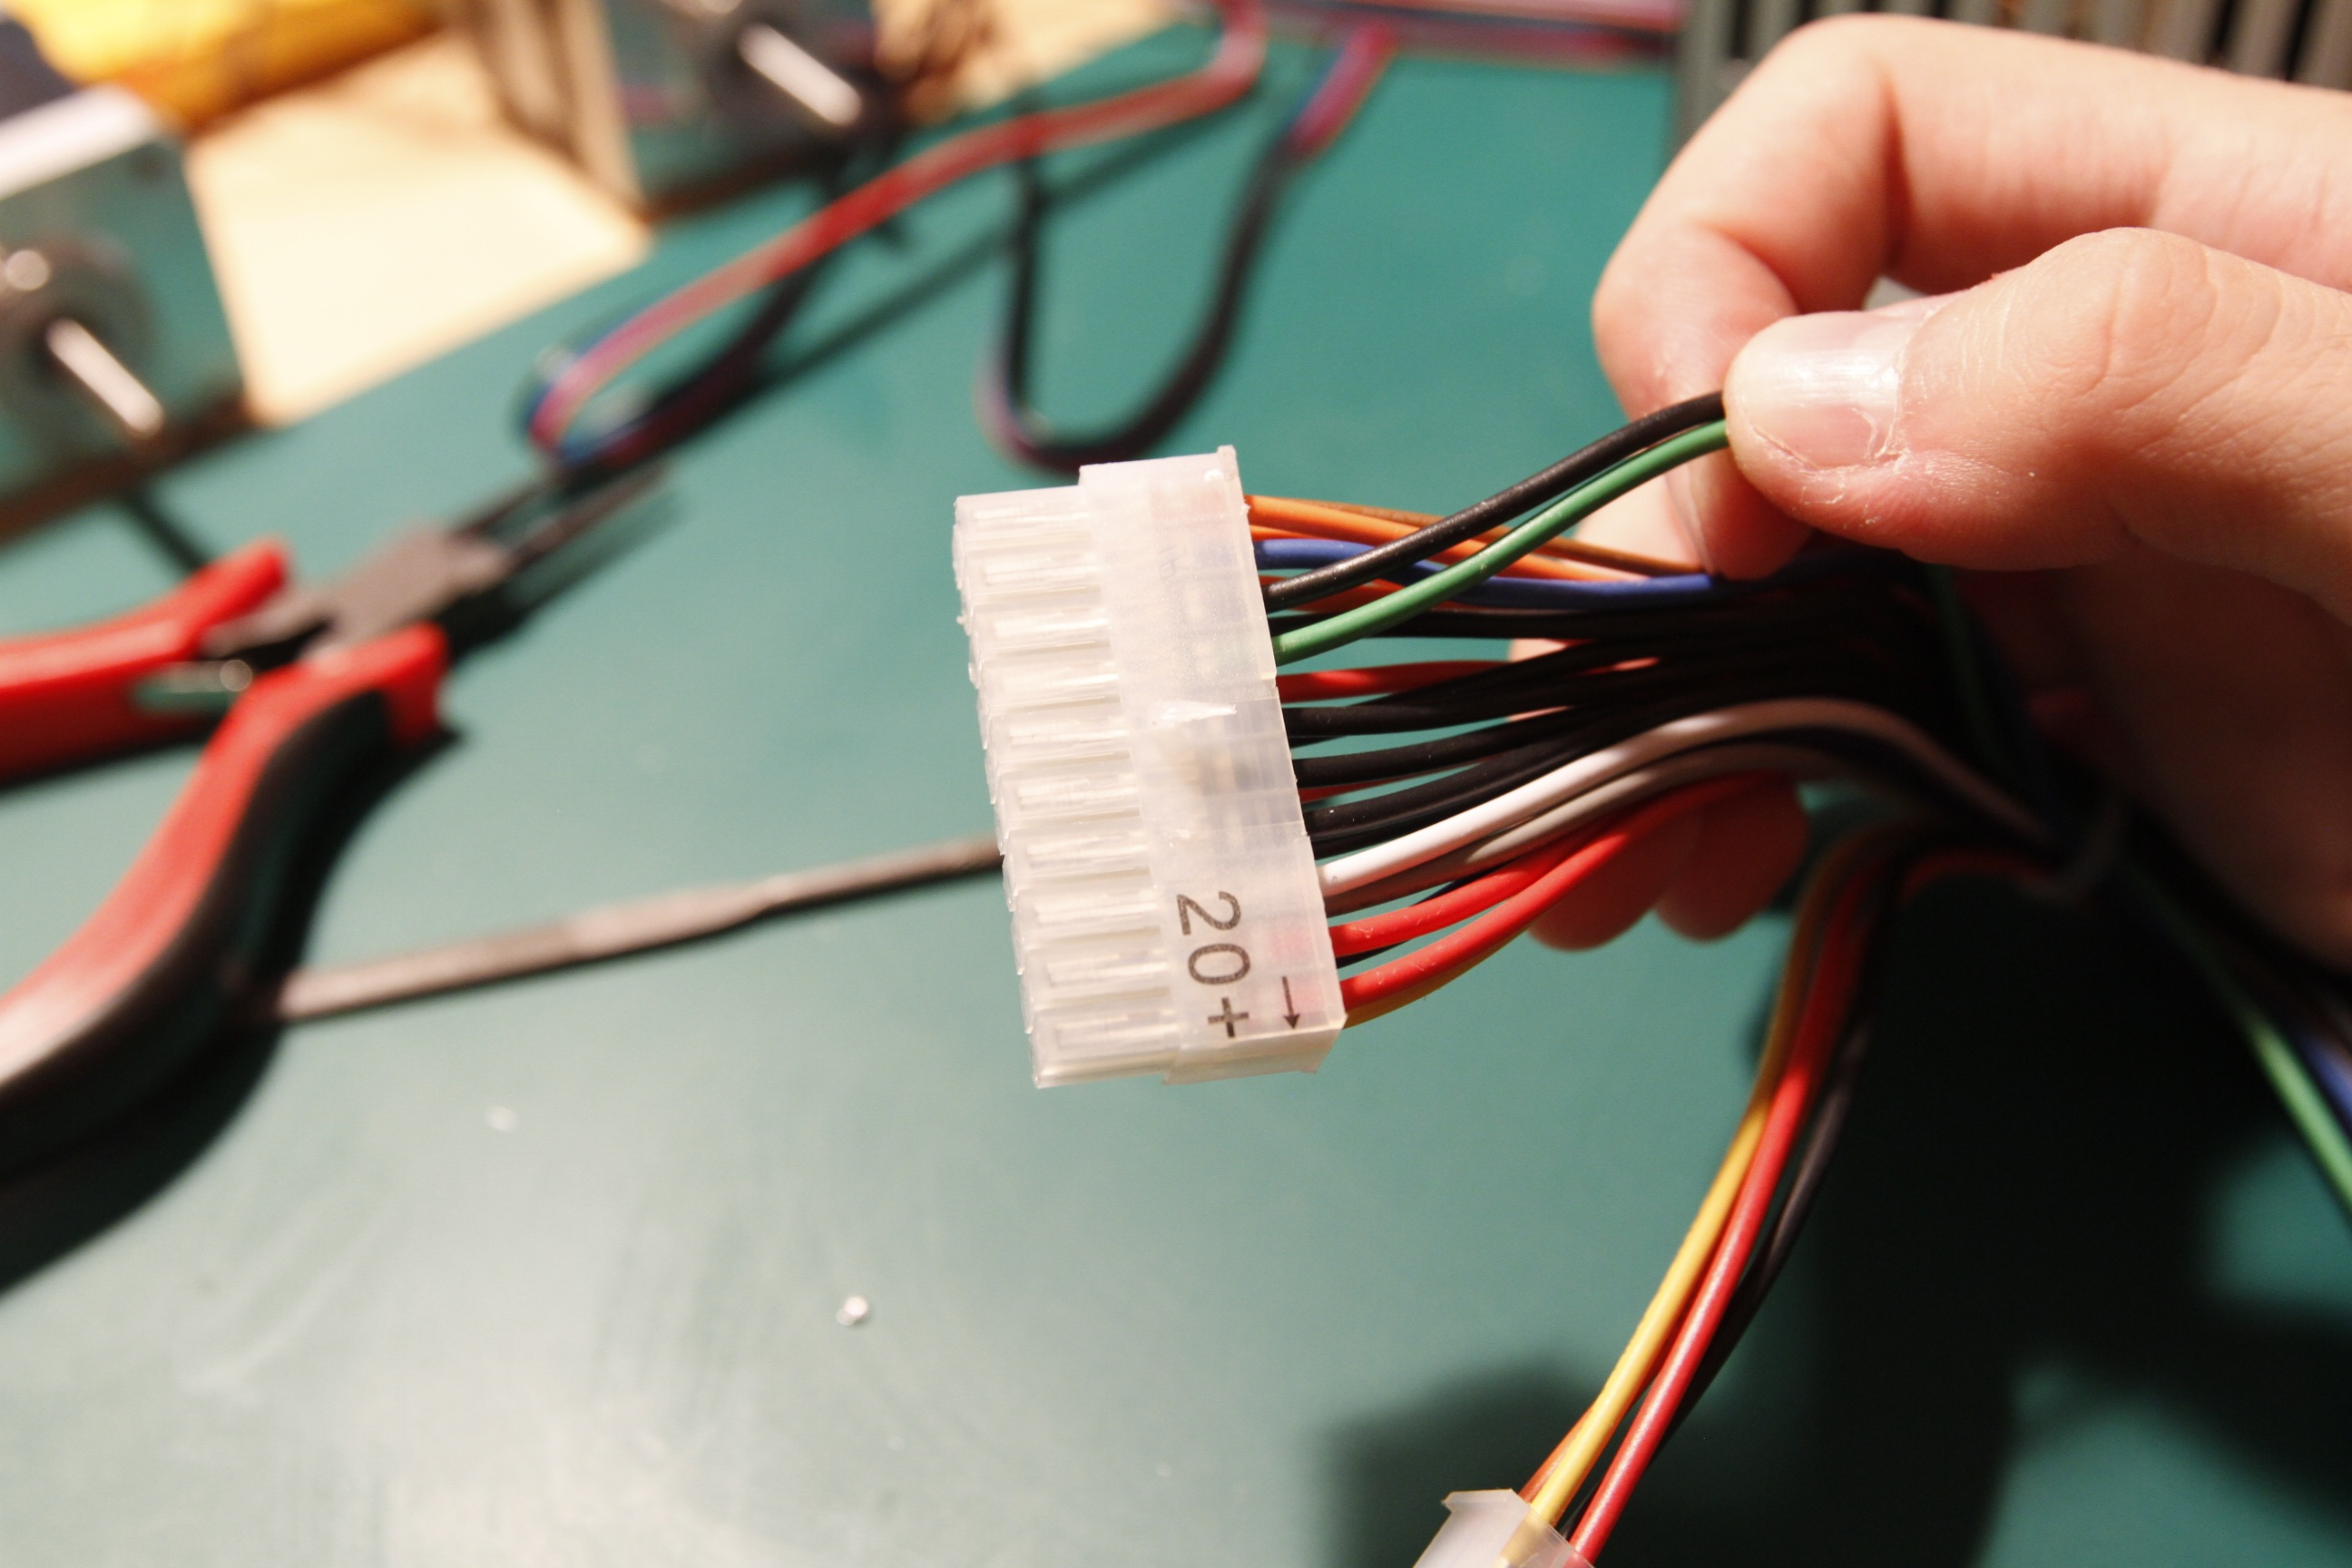
\includegraphics[width=\textwidth]{../../Fotos/20.jpg}
			                \caption{Cortocircuito en fuente }
			                \label{fig:atx.fuente}
			        \end{subfigure}
			        \begin{subfigure}[htb]{0.4\textwidth}
			                \centering
			                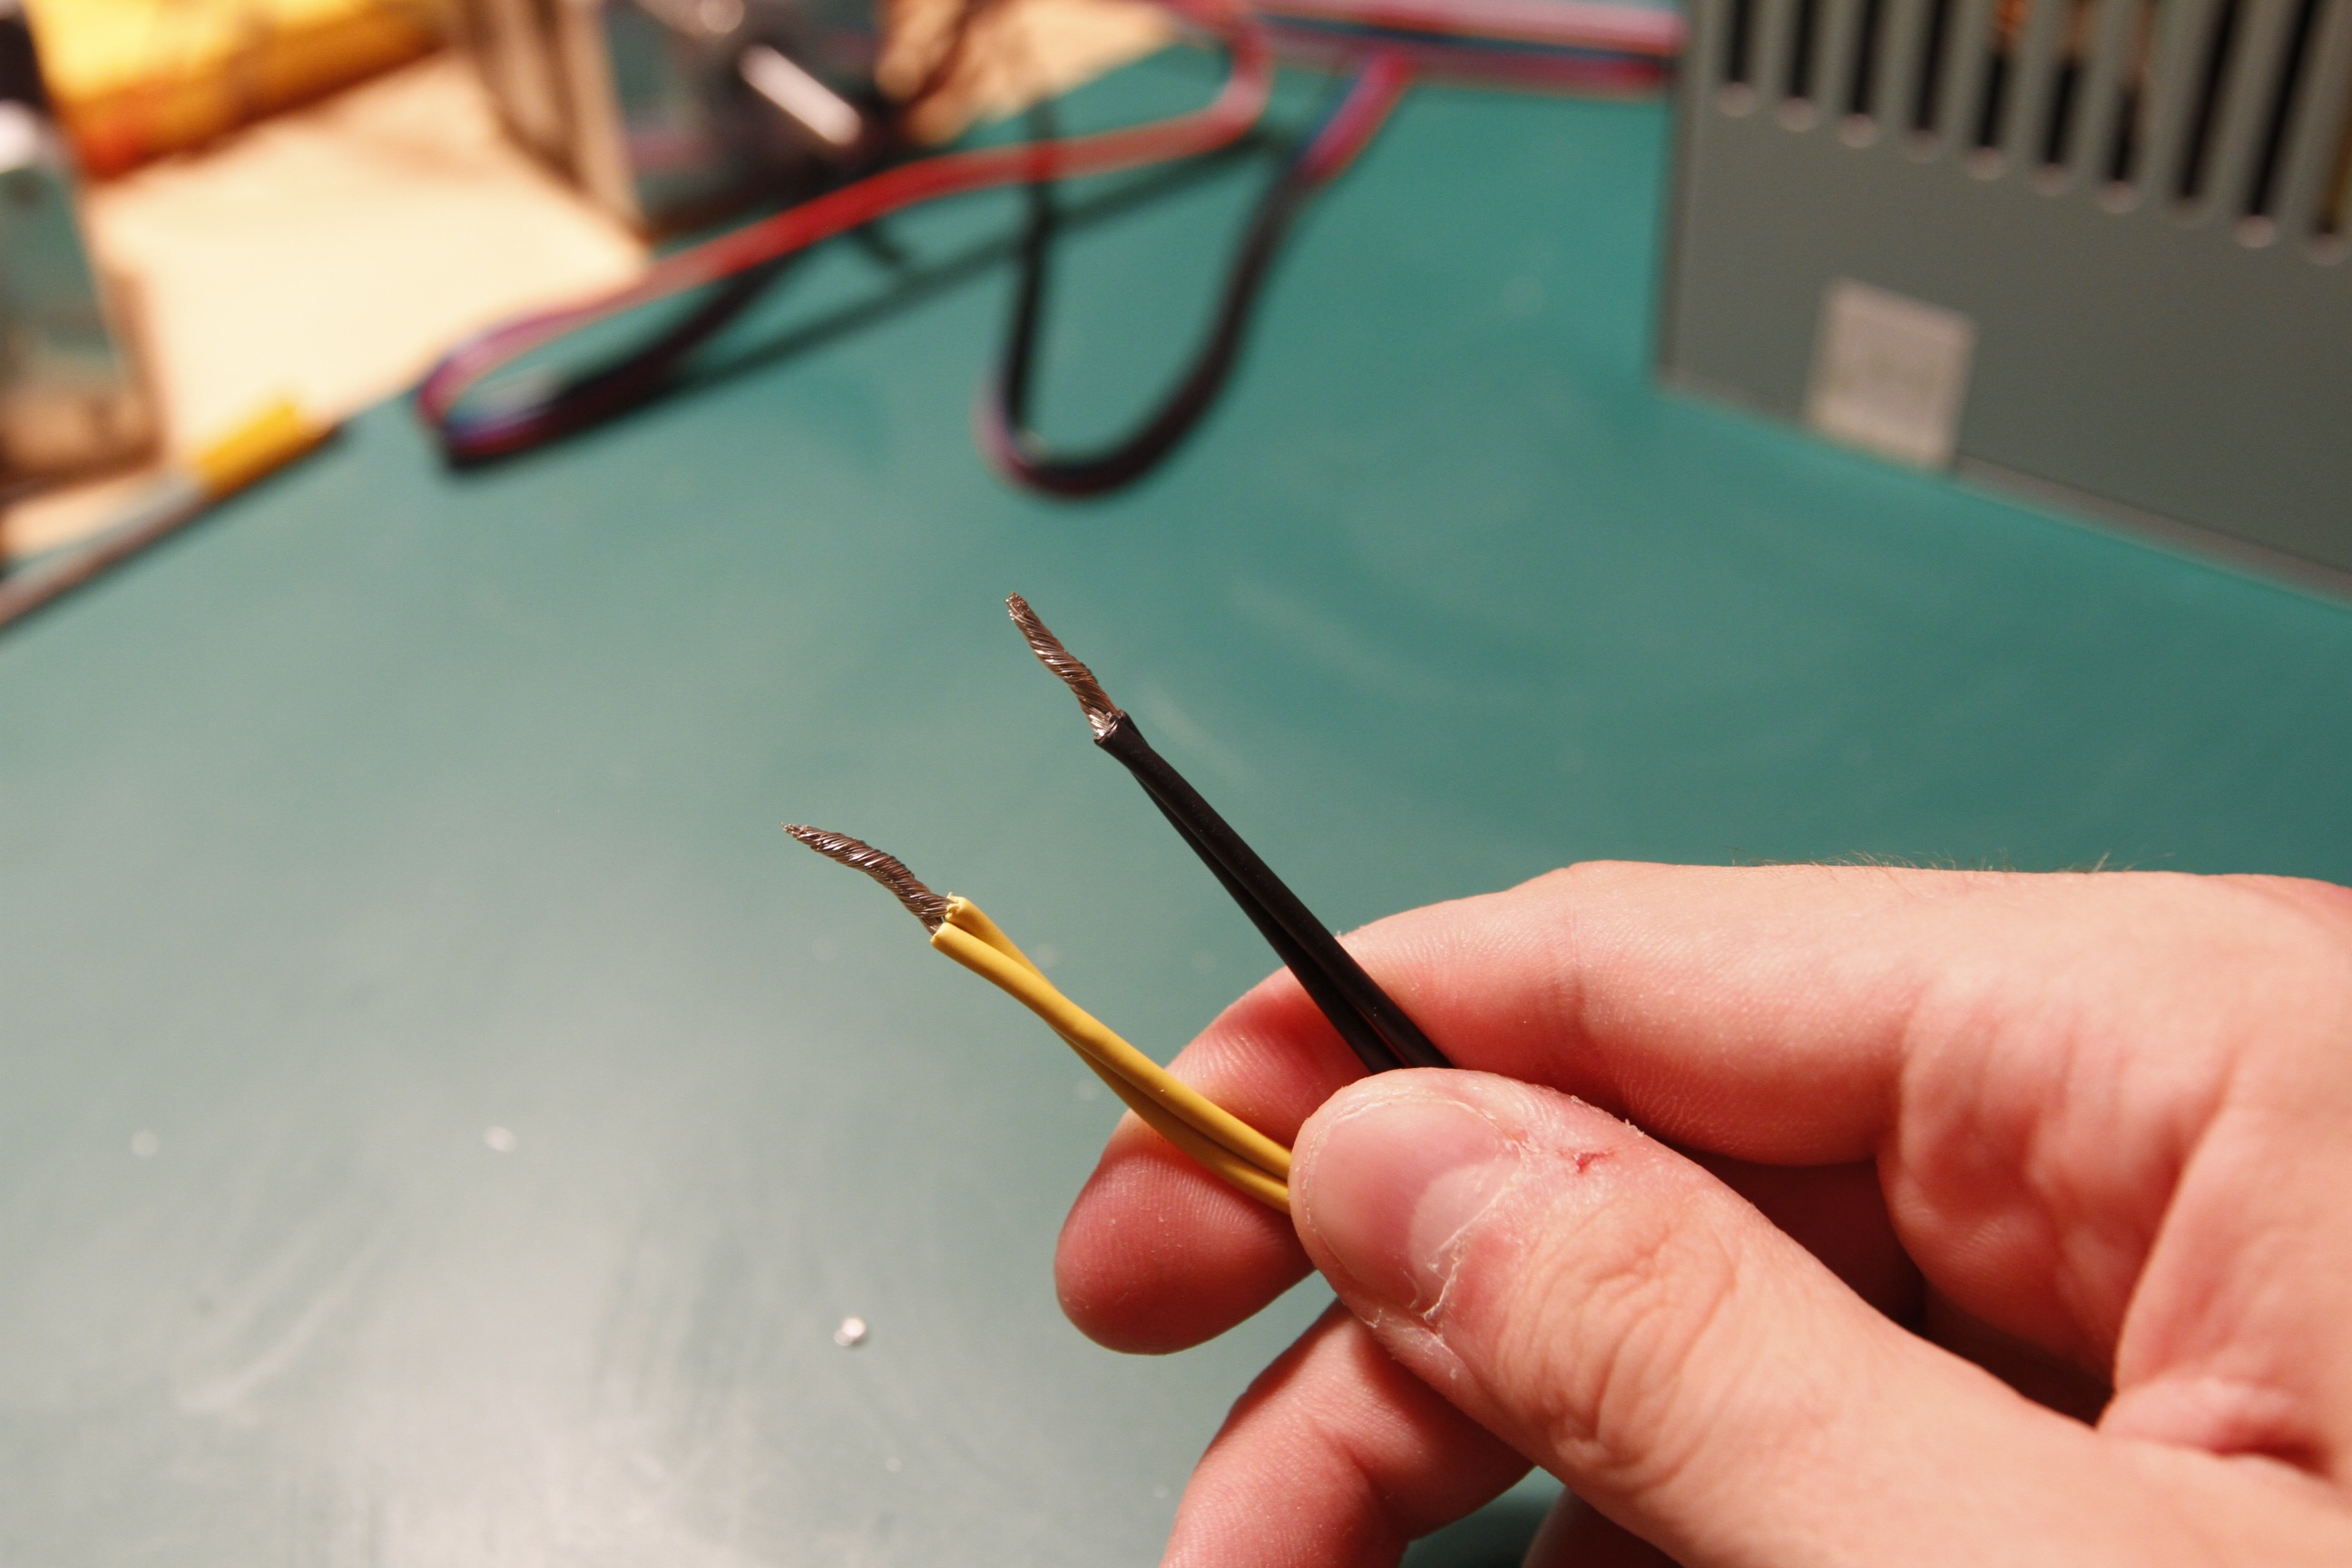
\includegraphics[width=\textwidth]{../../Fotos/21.jpg}
			                \caption{Cables de Vcc y GND}
			                \label{fig:vcc.fuente}
			        \end{subfigure}
			        \caption{Modificando Fuente de alimentación}\label{fig:fuente.alimentación}
			\end{figure}
			Seguidamente, conectaremos la fuente y el polímetro en modo amperios a la placa. Para ello nos ayudaremos del esquema siguiente:\\
			\begin{figure}[H]
				\centering
				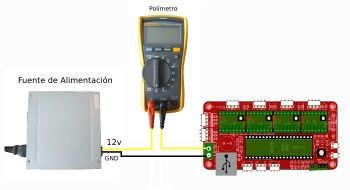
\includegraphics[width=0.6\textwidth]{../../Fotos/30.jpg}
				\caption{Esquemático sanguino.}
				\label{fig:amperimetro.sanguino}
			\end {figure}
Ahora realizaremos la primera conexión mediante pronterface a la placa. Para ello lo ejecutamos y nos cercioramos de que en \emph{Port} tenemos elegido el puerto al que tenemos conectado la electrónica, y tenemos seleccionada la velocidad que indicamos en marlin, por defecto 115200. Le damos a conectar y nos debería parecer algo similar a esto:\\
\begin{figure}[H]
	\centering
	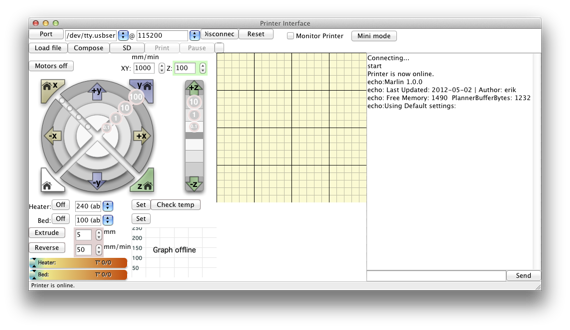
\includegraphics[width=1\textwidth]{../../Fotos/32.png}
	\caption{Pronterface.}
	\label{fig:pronterface}
\end {figure}
		Conectaremos un motor y el endstop al eje X en la placa y le daremos al botón Home X, de este modo el motor empezará a moverse buscando el endstop, en el momento que nosotros pulsemos el endstop se parará, si para que se mueva necesitamos mantener pulsado el endstop y cuando lo soltemos se para, necesitamos cambiar la lógica del endstop como vimos en la figura ~\ref{fig:endstop.marlin} página ~\pageref{fig:endstop.marlin} y en lugar de poner \textbf{\emph{false}}, poner \textbf{\emph{true}}. Una vez configurados correctamente los motores y los endstop, volveremos a darle al boton Home X está vez sin pulsar, y deberemos de moficiar en potenciometro del driver hasta que en el polímetro tengamos 200mA, si el motor se pará puede ser porque no le pase suficiente corriente, o porque haya llegado al final por software, volveremos a darle a Home hasta obtener los 200mA.\\
		\begin{figure}[H]
			\centering
			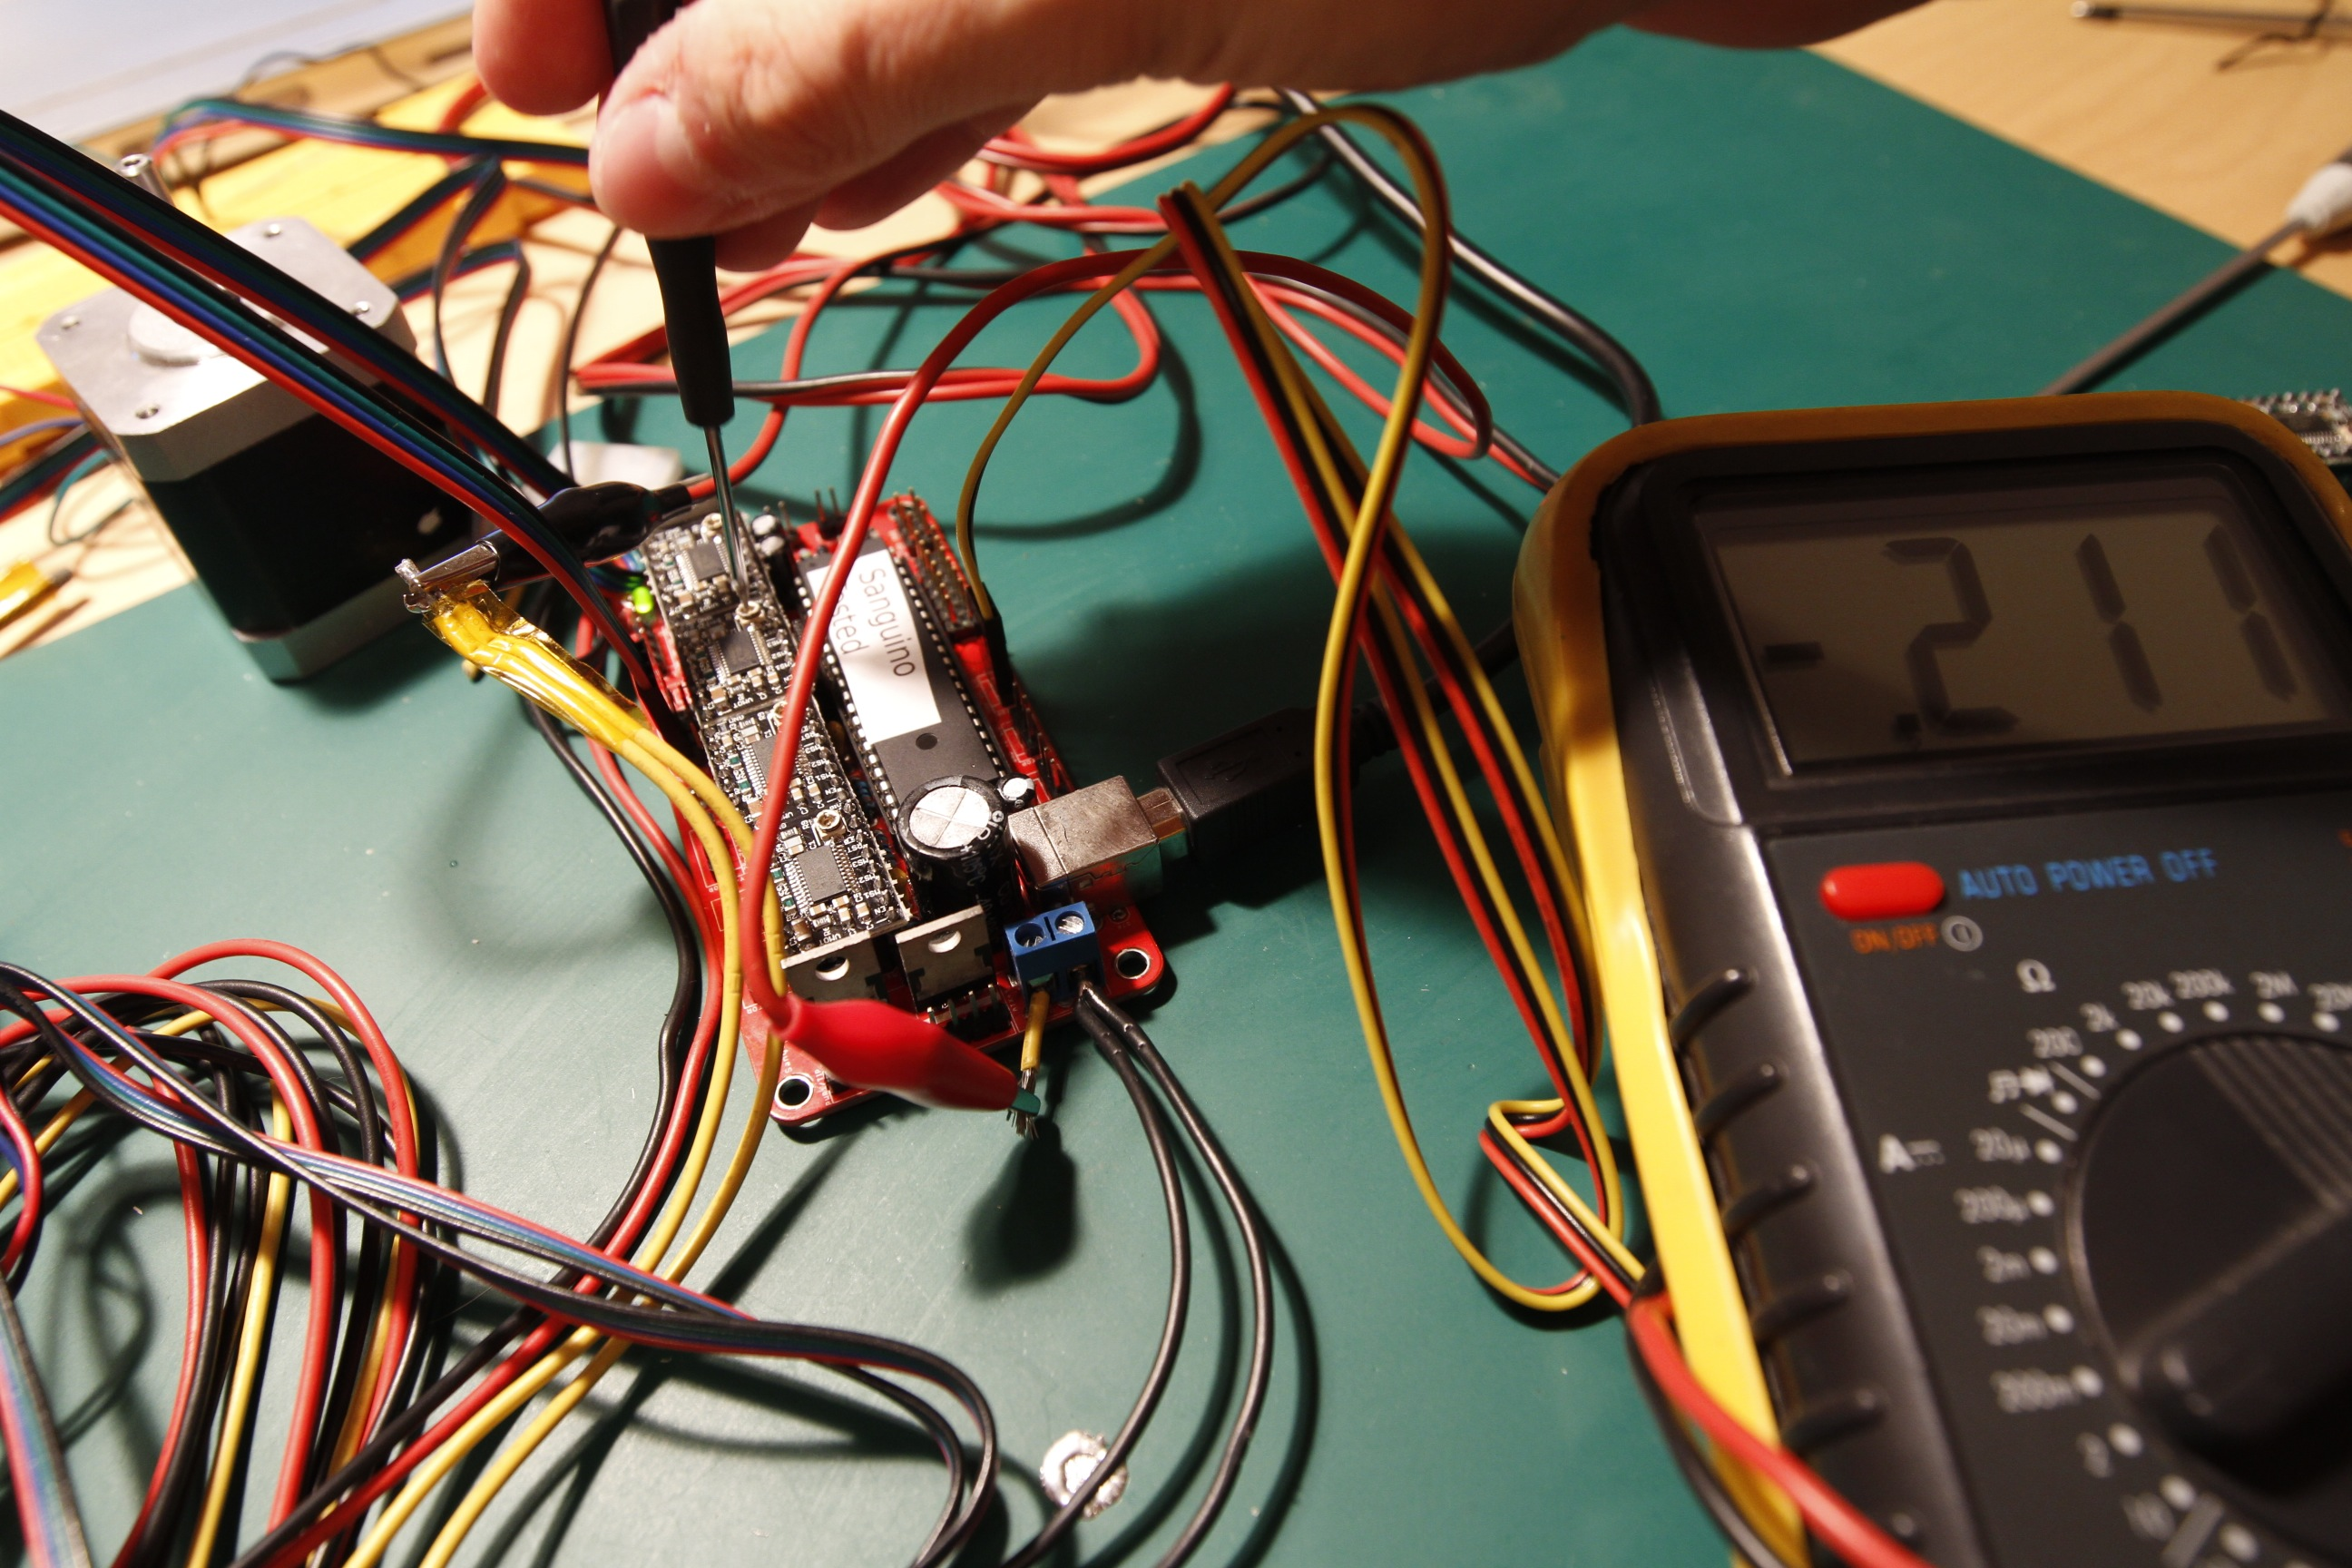
\includegraphics[width=0.5\textwidth]{../../Fotos/23.jpg}
			\caption{Calibrando stepstick.}
			\label{fig:calibrando.stepstick}
		\end {figure}
			Repetiremos esto con el eje Y, el eje Z y el extrusor. Para el eje Z será necesario colocar los dos motores y para el extrusor, debido a una protección por software el motor no se moverá, para ello colocamos el driver del extrusor donde iría colocado el del eje X y lo calibramos. Los amperios para cada driver están detallados en la tabla ~\ref{tab:amperios.stepstick}:
			\begin{table}[H]
				\centering
			\begin{tabular}{|c|c|}
			\hline
			Eje & Amperaje (mA) \\
			\hline
				X & 200 \\
			\hline
				Y & 200 \\
			\hline
				Z & 400 \\
			\hline
				Extrusor & 400 \\
			\hline
			\end{tabular}
			\caption{Amperaje de cada stepstick}
			\label{tab:amperios.stepstick}
			\end{table}